	\documentclass[preprint,11pt,authoryear]{elsarticle}
	\usepackage{amsmath}
	\usepackage[font=sf, labelfont={sf,bf}, margin=0cm]{caption}
	\usepackage[inline]{enumitem}
	\usepackage{epstopdf}   
	\usepackage[margin=1in]{geometry}
	\usepackage{lineno}
	\usepackage{placeins}
	\usepackage{subcaption}
	\usepackage{color}
	\usepackage{algorithm}
	\usepackage{algpseudocode}
	\usepackage{textcomp}
	\usepackage{graphicx}
	%\usepackage[section]{placeins} %prevents floats from appearing before their sections. web address  https://tex.stackexchange.com/questions/32598/force-latex-image-to-appear-in-the-section-in-which-its-declared
	\usepackage{float}
	
	\journal{Chemical Engineering Research and Design}
	\begin{document}
	\begin{frontmatter}
	\title{ NSF CDSE DRAFT 02}
	\author{Thor }
	\author{Gibbs }
	\author{Zeus }
	\author{the guy who invented sticky notes }
	\author{Santa Claus\corref{cor1}} 
	\ead{santaclaus}
	\cortext[cor1]{Corresponding author}
	\address{North Pole department of ice and snow Fwding address - Department of Chemical and Biochemical Engineering, Rutgers, The State University of New Jersey, Piscataway, NJ, USA 08854}
	\begin{abstract}
	 abstract text goes here ...
	\end{abstract}
	\begin{keyword}
	Population balance model \sep heteroaggregation \sep alginate  \sep chitosan \sep oppositely charged
	\end{keyword}
	\end{frontmatter}
	\linenumbers
	
	\section{Introduction \& Objectives} 

	\par Half of all industrial chemical production is carried out using particulate processes (\cite{seville1997}). Important products that are produced using particulate processes include detergents, aerosols, fertilizers, and pharmaceuticals. Particulate processes have complex phenomena due to the chaotic microscale behaviour of individual particles in the system that determine the bulk behaviour of the system. Due to the complex nature of these processes there is a lack of governing equations which can accurately describe them (\cite{sen2013}). As a result industries such as pharmaceuticals use expensive heuristic studies and inefficient operational protocols with high recycle ratios to meet strict regulatory standards (\cite{Ramachandran2009}). In an effort to cut costs and improve efficiencies there is a high demand for accurate models that can be used for process design and control systems.   
	\par Discrete element methods (DEM)(\cite{Cundall1979}) have proven to be an accurate way to model a bulk material using microscale particle level interactions. The downside to these models is that they take large amounts of time to solve. Another more computationally efficient, but less accurate, technique used for these systems are population balance models (PBM). To achieve high levels of accuracy without the long simulation times of DEM there have been numerous works on hybrid PBM-DEM methods \citep{Barrasso2015cerd}.
	\par  The idea of parallelization to reduce the amount of time required has been employed by various researchers in the past. \cite{Gunawan2008} used high-resolution finite volumes solution methods for the parallelization of their PBM. \cite{Gunawan2008} performed load balancing effectively by decomposing the internal coordinates of their PBM. They acheived speed improvements upto 100 cores on one system size, but was not tested for models with more dimensions. Moreover, they mentioned that the parallelisation could be improved using shared memory processing. \cite{Bettencourt2017} took a hybrid approach towards the parallelization of the PBM using both Message Parsing Interface (MPI) and Open Multi-Processing. The hybrid parallelisation helped achieve a speed up of about 98\% over the serial code. \cite{Prakash2013a},\cite{Prakash2013b} used the inbuilt Parallel Computation Toolbox (PCT) in Matlab to parallelize their PBM on lower number of cores, but this faced the shortcomings of Matlab's internal processing and could not achieve the speed improvements of parallelistion of a program if it were written in a native programming language like C or FORTRAN. 
	\par  LIGGGHTS is an open-source software used to perform DEM simulations. This package natively supports MPI for parallelizing the simulation by static decomposition which partitions space such that the area of communication between the the MPI ranks is minimized. \cite{kacianauskas2010} used load balancing methods similar to a static decompostion and observed that this works well for a mono-dispersed system but the computational effort increases for simulations for poly-dispersed material. \cite{Gopalakrishnan2013} also reported a speed increase and a parallel efficiency of about 81\% in their CFD-DEM simulation. LIGGGHTS could not take advantage of shared memory interfaces since it did not support OpenMP. \cite{Berger2015} implemented hybrid parallelization methods for the particle-particle interaction and the particle-wall interaction modules in LIGGGHTS and also used the Zoltan library \citep{Boman2012} developed by Sandia National Laboratories for dynamic load balancing. They achieved a speed improvement of about 44\% for simulations performed on higher number of cores, but there was no significant speed improvement for smaller core counts.
	%\par Use of parallel techniques by scientists have helped reduce the amount of time required to solve computationally heavy tasks into a array of smaller and more manageable tasks, which are solved simultaneously in various smaller processes. 
	\par Some of the potential benefits of using HPCs in the pharmaceutical industry include really high accuracy for parameter estimation, on-line modelling of continuous processes, better control of processes. This would lead lesser production costs leading to cheaper drug for the consumer.
	
	    \subsection{Objectives}
	    \par The main objective of this study was to develop new techniques to parallelize our model and use high perfomance computing (HPC) equipment in order to reduce the computation times for the linked DEM-PBM simulations. Specific objectives of each individual study are listed below: 
	    \begin{itemize}
	    \item Developed a 4-Dimensional PBM that is parallelized using hybrid techniques (MPI + OpenMP)  for optimal utilization of modern high performance computing equipment.
	    \item LIGGGHTS (MPI-only implementation) has been used to perfrom Discrete Element Model (DEM) simulations to  model the micromechanics of the Lodgitech granulator. 
		\item These 2 techniques were linked uni-directionally to provide an accurate model of the granulator.	    
	    \end{itemize}

	

	\section{Background \& Motivation}
	
	  %\subsection{Particulate Processes}
	  \par Particulate processes are ones in which a system of discrete species exist, such as granules or catalyst pellets, that undergo changes in average composition, size, or other pertinent properties. Such processes are prevalent in the pharmaceutical industry. These processes have great oppurtunities in better equipment design, process efficiency and scale-up (\cite{Ketterhagen2009}). 
	     
  %\par as result use time consuming and expensive heuristics or inefficient operation protocol  dotdotdot also reason most blah done in batch mode still bec continuous mode compounds complexity of these systems \par will need to switch to continuous etc  
  %\par segway with need to better understand these systems from a modelling/theory point of view dotdotdot QbD etc 
	  
	  \subsection{Modeling}
		\par The quality by design (QbD) concept i.e, theoritically modelling the process for better quality of the product is being implemented by the pharmaceutical industry due to its cost benefits. Also, the paradigm shift of the industry towards continuous manufacturing, emphasizes the need to model these processes more accurately. This further helps develop better control stratergies for the process.The modelling of these processes is more time consuming and computationally expensive when compared to a fluid systems since the particles are considered as individual entities rather than a continuum like in fluid systems. The models discussed represent the particle-particle interaction at meso and micro-scale.	  
	    \subsubsection{Discrete Element Modeling (DEM)}
	    \par Discrete Element Method is a simulation technique used to monitor the behaviour of each particle as a separate entity compared to other bulk continuum models. This method tracks the movement of each of the particles with in the space, records the collisions of each particle with the geometry as well as with each other and it is also subject to other force fields like gravity (\cite{Barrasso2015cerd})  This model is based on the Newton's laws of the motion and is expressed as in Equations \ref{eqn:bkgd_dem_n2law} and  \ref{eqn:bkgd_dem_forcebal} : \\
	\begin{align}
	m_i\frac{dv_i}{dt} &= F_{i,net} \label{eqn:bkgd_dem_n2law} \\
	F_{i,net} &=  F_{i,coll} +  F_{i,ext} \label{eqn:bkgd_dem_forcebal}
	\end{align}
	\par  In the above equations $m_i$ represents the mass of the particle, $v_i$ represents the velocity of the particle, $F_{i,net}$  represents the net force on the particle, forces on the particle due to collisions and other external forces are represented in $F_{i,coll}$ $F_{i,ext}$ respectively.
	\par The distance between each particle calculated at every time step and if the distance between two particles is less than the sum of the radii (for spherical particles)  a collision between the two particles is recorded. The tolerance for overlap is low in the normal as well as the tangential direction (\cite{Cundall1979}). Microscale DEM simulations are computationally demanding and simulations may take upto several days to replicate a few seconds of real time experiments. Many methods have been implemented to increase the speed of these simulations, such as scaling by increasing the size of the particles. These approximations are good in understanding the physics of the system but are not directly applicable to process-level simulations. 
	%\par Commercially available softwares for DEM simualtions have not been able to take advantage of the recent advances in computing power in terms of supercomputers. This
	\par Thus, this method for granular powder is usually replaced by Population Balance Method which is a much quicker approximation as it is a bulk model.  

	    \subsubsection{PBM}
	    \par Population balance models (PBM) predict how groups of discrete entities will behave on a bulk scale due to certain effects acting on the population with respect to time (\cite{ramkrishna2014}). In the context of process engineering and granulation, population balance models are used to describe how the number densities, of different types of particles, in the granulator change as rate processes such as aggregation and breakage reshape particles (\cite{Barrasso2013}). A general form of population balance model is shown here as equation \ref{eqn:bkgd_pbm_general}.
	    
	    \begin{align}
	    \frac{ \partial}{\partial t}F(\textbf{v},\textbf{x},t) +& \frac{\partial}{\partial \textbf{v}}[F(\textbf{v},\textbf{x},t)\frac{d\textbf{v}}{dt}(\textbf{v},\textbf{x},t)] + \frac{\partial}{\partial \textbf{x}}[F(\textbf{v},\textbf{x},t)\frac{d\textbf{x}}{dt}(\textbf{v},\textbf{x},t)] \notag\\
	    &= \Re_{formation}(\textbf{v},\textbf{x},t)+\Re_{depletion}(\textbf{v},\textbf{x},t)+\dot{F}_{in}(\textbf{v},\textbf{x},t)-\dot{F}_{out}(\textbf{v},\textbf{x},t)
	    \label{eqn:bkgd_pbm_general} 
	    \end{align}
	    
    \par In equation (\ref{eqn:bkgd_pbm_general}), $\textbf{v}$ is a vector of internal coordinates. For modelling a granulation process $\textbf{v}$ is commonly used to describe the solid, liquid, and gas content of each type of particle. The vector $\textbf{x}$ represents external coordinates, usually spatial variance. For a granulation process this  account for spatial variance in the particles as they flow along the granulator.
    \par PBM extensively used for calculating granulation rate processes (e.g.~aggregation, consolidation and breakage) but it cannot provide information related to mechanistic kernels of these rate processes i.e.~collision frequency, collision efficiency, particle velocity etc.~(\cite{sen2014}). On the other hand, DEM able to determine these entities. A hybrid model for one-way coupling has been reported for continuous mixing (\cite{sen2013} \& \cite{sen2013b}) and is discussed in later section.
	    
	    
	
	    \subsubsection{Multi-physics models}
		\par The use of multi-physics models has recently been adapted to understand the behaviour of particle systems. These models help understand the physics of the system at various scales \textit{i\.e\.} micro, meso and macro scale(\cite{sen2014}). Particle process dynamics have been inferred from coupling of various physics models \textit{viz.} Computational Fluid Dynamics (CFD), DEM and PBM. Earlier works from \cite{sen2014} and \cite{Barrasso2015cerd} have successfully predicted process dynamics of the granulation process.
		\par In this work, a coupling of DEM and PBM was implemented. The PBM gives meso scale information and the DEM gives particle scale information. Combination of these two methods help comprehend the process dynamics with more accuracy. The calculations involved due to the number of particles involved in the DEM process as well as PBM become very computationally heavy. The recent development in the design of CPUs and increasing number of cores in the CPU, it makes sense to utilize them to make the simulations faster. Thus, implementation of various parallel computing techniques was employed in this work to help improve the simulation times.  
	
	
	  \subsection{Parallel Computing and Computer Architectures}
	    %\subsubsection{Overview}
	    \par The goal of parallel computing is to distribute large amounts of computation across many compute cores to solve problems faster (\cite{wilkinson2005}).
		\subsubsection{Computer Architecture}
	    \par Parallel programs are commonly run on computer clusters. Computer clusters are a collection of nodes interconnected by a high speed communication network for message passing from one node to another. Analogously to a conventional PC each node as one or more CPUs and RAM. Commonly nodes are manufactured with two CPUs, each CPU is a multi-core meaning it has multiple compute cores that each can carry out calculations separately from one another. CPUs also have built in memory called cache that is much faster than RAM which is why for optimal performance cache utilization should be favoured over RAM when possible. On a node memory is divided by CPU sockets, so each CPU has direct access to memory local to its own socket, but accessing memory on another socket is much slower \cite{Jin2011}. For this reason data that is needed for computation should be stored locally to the CPU that needs it.  
	    \par Two common classes of computer architecture classified by memory locality features are distributed memory systems and shared memory systems. These two classes co-exist in a cluster, thus providing the benfits of each. All the nodes share memory using explicit message passing while each has its own independent memory. The cores on each node can access data from the shared memory without any explicit message passing statements from the user. While designing a parallel program all these aspects need to be considered for optimal perfomance of the code (\cite{Adhianto2007}).
	    %Computer architectures are often classified by memory locality features. There are two distinct classes, distributed memory systems and shared memory systems. A cluster is a combination of the two classes. Each node operates its memory independently of the other nodes and explicit message passing is needed to share memory between nodes. While the cores on a node can operate in shared memory mode since memory updates can be made without explicit message passing statements from the user. All of these aspects of the computer architecture should be considered when designing a parallel program for the best performance  \textcolor{cyan}{maybe reword better to make more like CACE paper}.
		
	    \subsubsection{Parallel Application Program Interfaces}
	    \par Message Passing Interface (MPI) is a common parallel computing application interface standard. MPI is used for distributed memory parallel computing, this is because MPI will operate every MPI process as a discrete unit that does not share memory with the other processes unless explicit message passing is used. Even on shared a single node where the hardware is supports shared memory computing, MPI will still operate it in a distributed memory fashion \cite{Jin2011}. Operating all cores as distinct units also means they each need their own copy of all variables used for computation which results in a large overall memory foot print compared to a same system if it was operated in shared memory. 
	    \par Open Multi-Processing (OMP) is another application program interface stand for parallel computing. OMP is used for shared memory and can take advantage of shared memory systems which can result in much faster computation. It does not work well on distributed systems though. This prevents it from being used to efficiently carry out computations across multiple nodes of a cluster simultaneously \cite{Jin2011}. 
	    \par Since MPI is preferred for distributed computing and OMP is better for shared computing many individuals have studied the performance of MPI vs MPI+OMP methods and many studies have used MPI+OMP for scientific computation for improved performance. Often times a trade of is made between optimizing a program for performance and trying to make it flexible enough to run on many different computer architectures. A summary of some works addressing MPI+OMP methods for scientific computing and architecture features and concerns can be found in \cite{Bettencourt2017}. In the conclusion to the work by \cite{Bettencourt2017} it was found that hybrid methods for PBMs allow the code flexibility for different architectures while still maintaining good performance.  In the work of \cite{Bettencourt2017} only the external(spatial) coordinates of the PBM were parallelized. In this current work external and internal(compositions) calculations are parallelized.% \textcolor{cyan}{comment about how int and ext pll methods means better model for xyz reasons dotdotdot helps to explicitly say reason} 
	      
	
	
	\section{Methods}
	
	  \subsection{DEM}
	    \subsubsection{LIGGGHTS}
	    	\par LAMMPS Improved for general granular and granular heat transfer simulations (LIGGGHTS\textsuperscript{\textregistered} v3.60) (\cite{Kloss2012}) developed by DCS computing was used for all the simulation performed in this study. Edits were made to the compute\_contact\_atom source file to obtain particle $-$ particle collisions. The aforementioned version of LIGGGHTS was compiled using the mvapich (mvapich2 v2.1) and intel (intel v15.0.2) compilers with the -o3 optimisation option as well as an option to sideload the process to the Xeon phi co-processors was added. The studies were performed on STAMPEDE supercomputer located at Univeristy of Texas, Austin. The hardware configuration of each node consists of 2 8-core Intel Xeon E5-2680 processors based on the Sandy Bridge architecture, 32 gb of memory with QPI interconnects at 8.0 GT/s PCI-e lanes.

	        
	    \subsubsection{Geometry}    
	    %\par \textcolor{red}{check other file Charles uploaded to see if that one was more "journal ready"}
	    
	    \par In this study, the L\"{o}dige CoriMix CM5 continuous high shear granulator has been studied. Its geometry was developed using the SolidWorks$^{TM}$ (Dassault Syst\`{e}mes). This granulator consisted of a high speed rotating element enclosed within a horizontal cylindrical casing. The casing (shown in Figure \ref{fig:mthdsDemCharlesGranShell}) consists of a cylinder with diameter of 120 mm at the inlet and 130 mm at the outlet and having a total length of 440 mm. A vertical inlet port is provided at one end of the casing and an angled outlet port is provided at the larger end of the case. 
	
	      \begin{figure}[H]
	      \centering
	      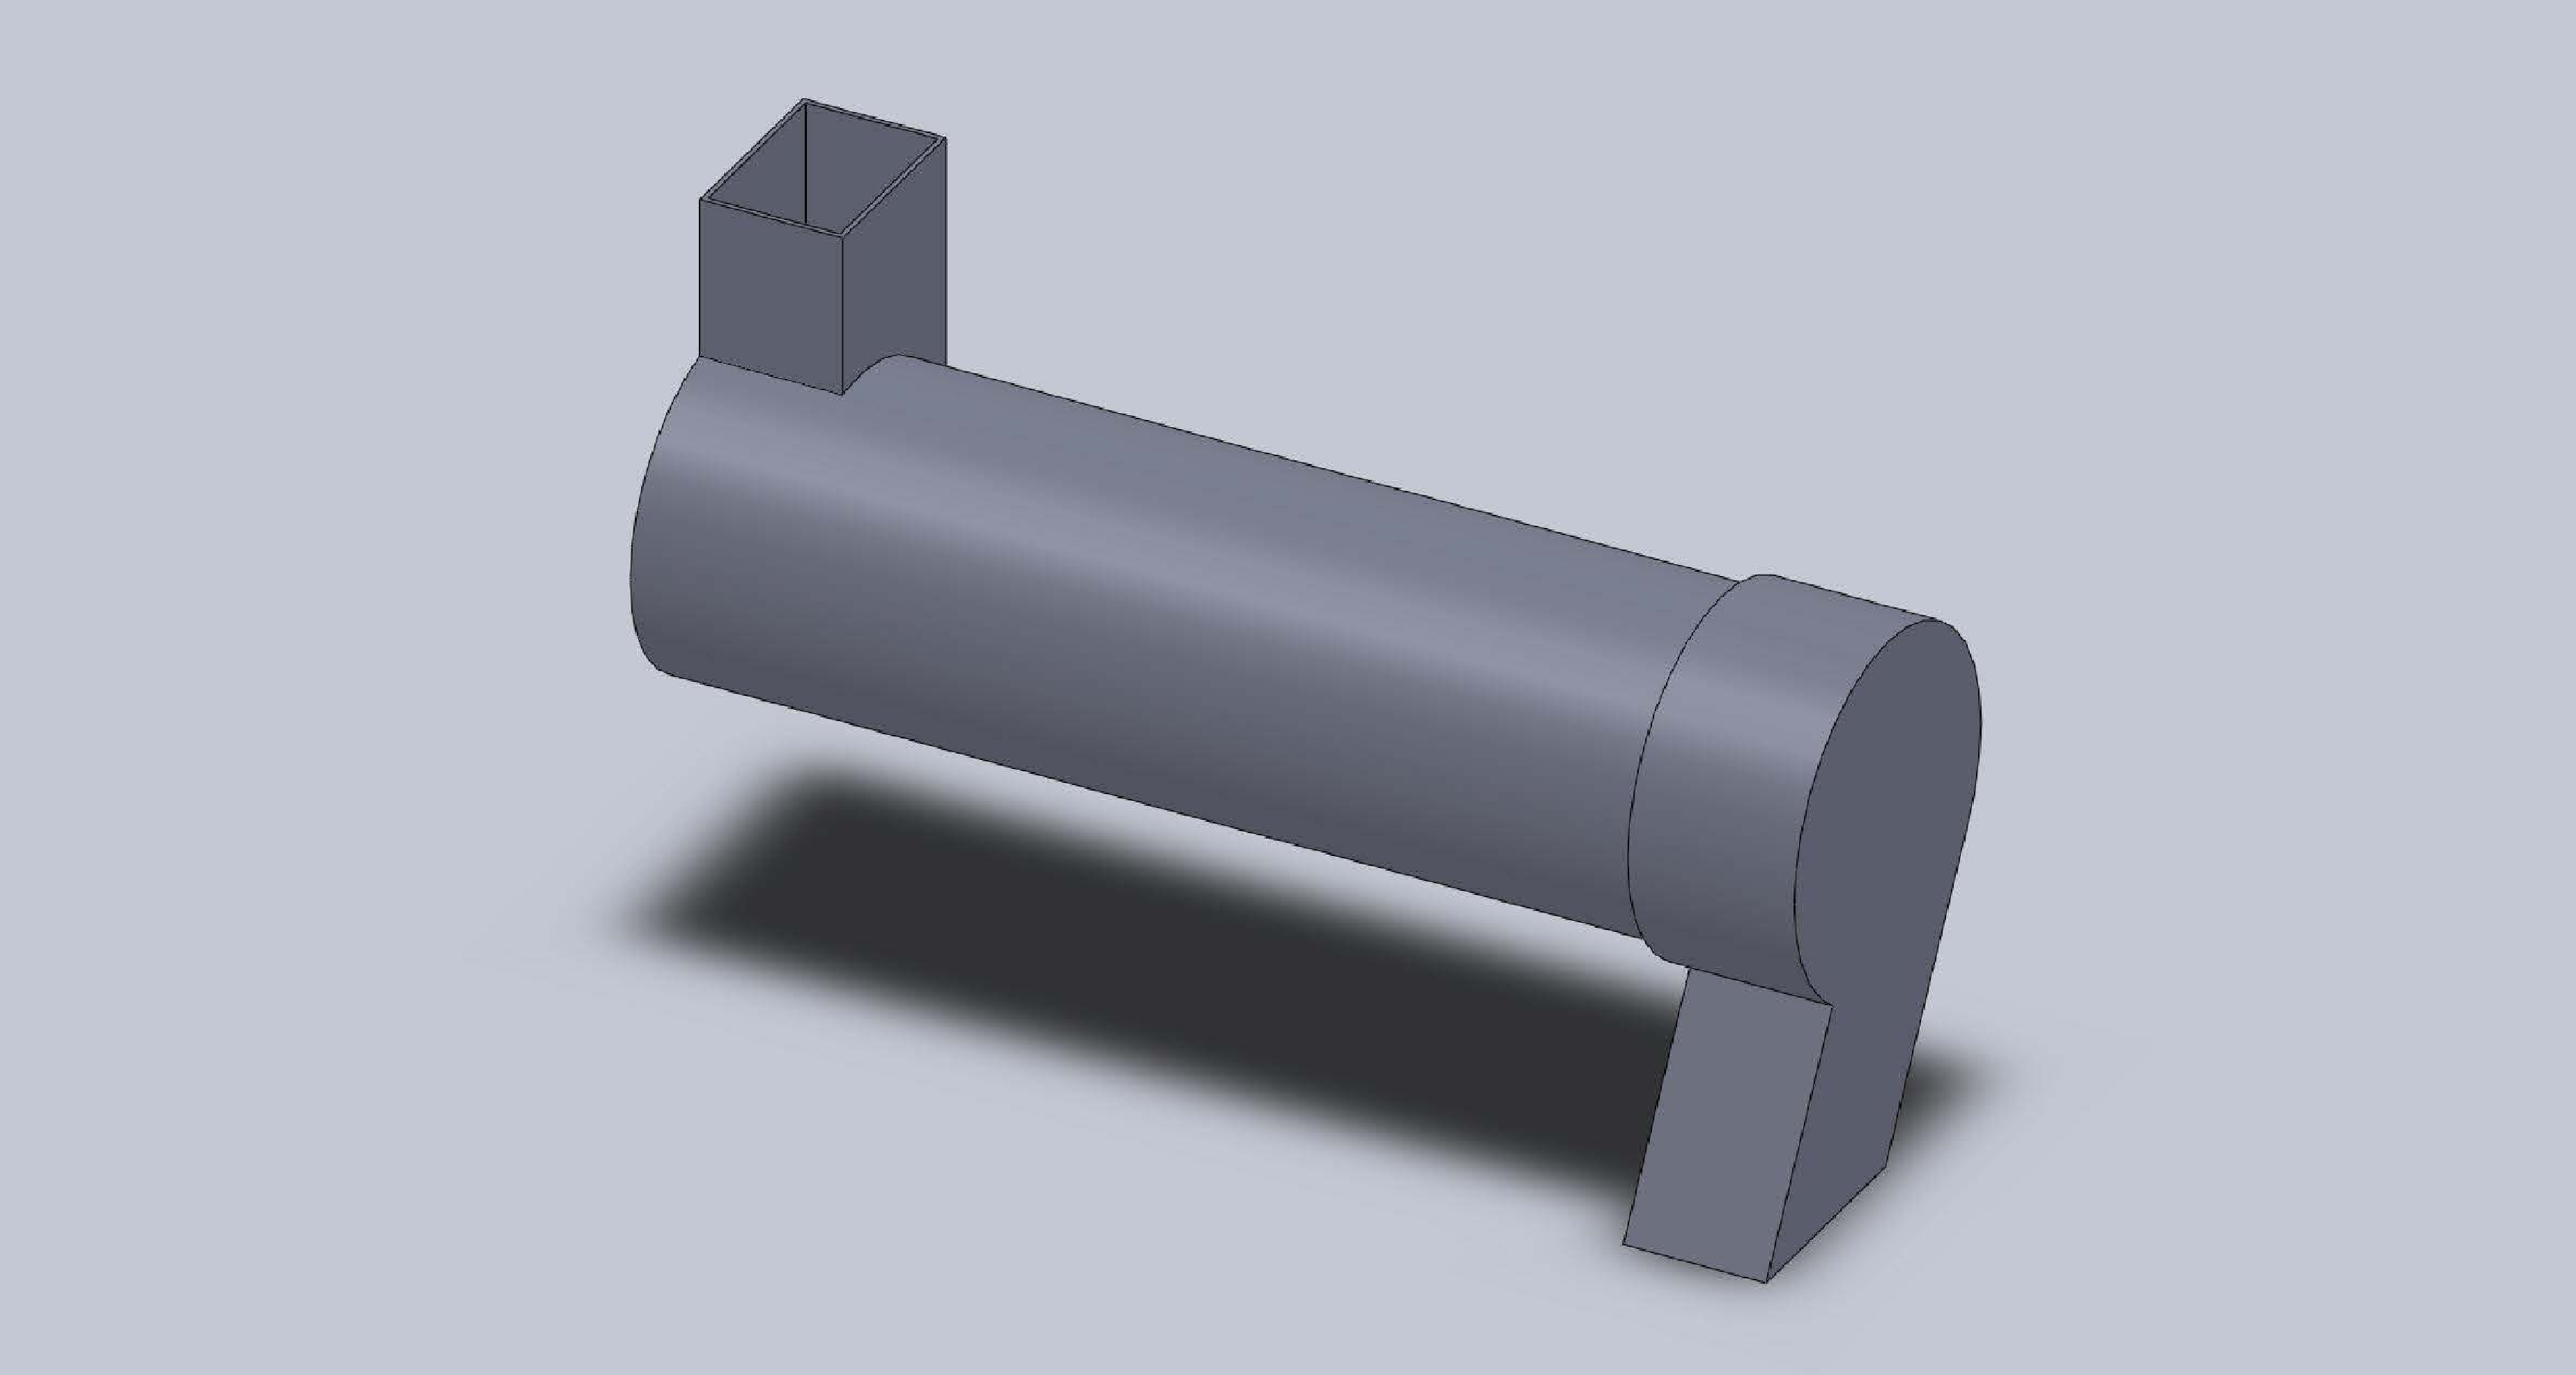
\includegraphics[scale=0.2]{shell_final_pic.pdf}
	      \caption{ Shows an isometric view of the granulator casing.}
	      %\caption{hello yuktesh}
	      \label{fig:mthdsDemCharlesGranShell}
	      \end{figure}
	   
	    \par  The impeller consists of a cylindrical shaft of length 370 mm and diameter 68 mm with four flattened sides 15 mm wide running along the axis. The blades are placed on these flattened sides as shown in figure \ref{fig:mthds_dem_charles_impeller}. There are three different blade elements on the shaft (figure \ref{fig:mthds_dem_charles_impeller}). At the granulator inlet, there are 4 paddle shaped feed elements following which there are 20 tear drop shaped shearing elements  and finally 4 trapezoidal blades near the exit. All these elements are placed in a spiral configuration. The final configuration of the granulator is shown in figure \ref{fig:mthds_dem_charles_fig5pt3and4_blades_n_isometric}.
	
	      \begin{figure}[H]
	      \centering
	      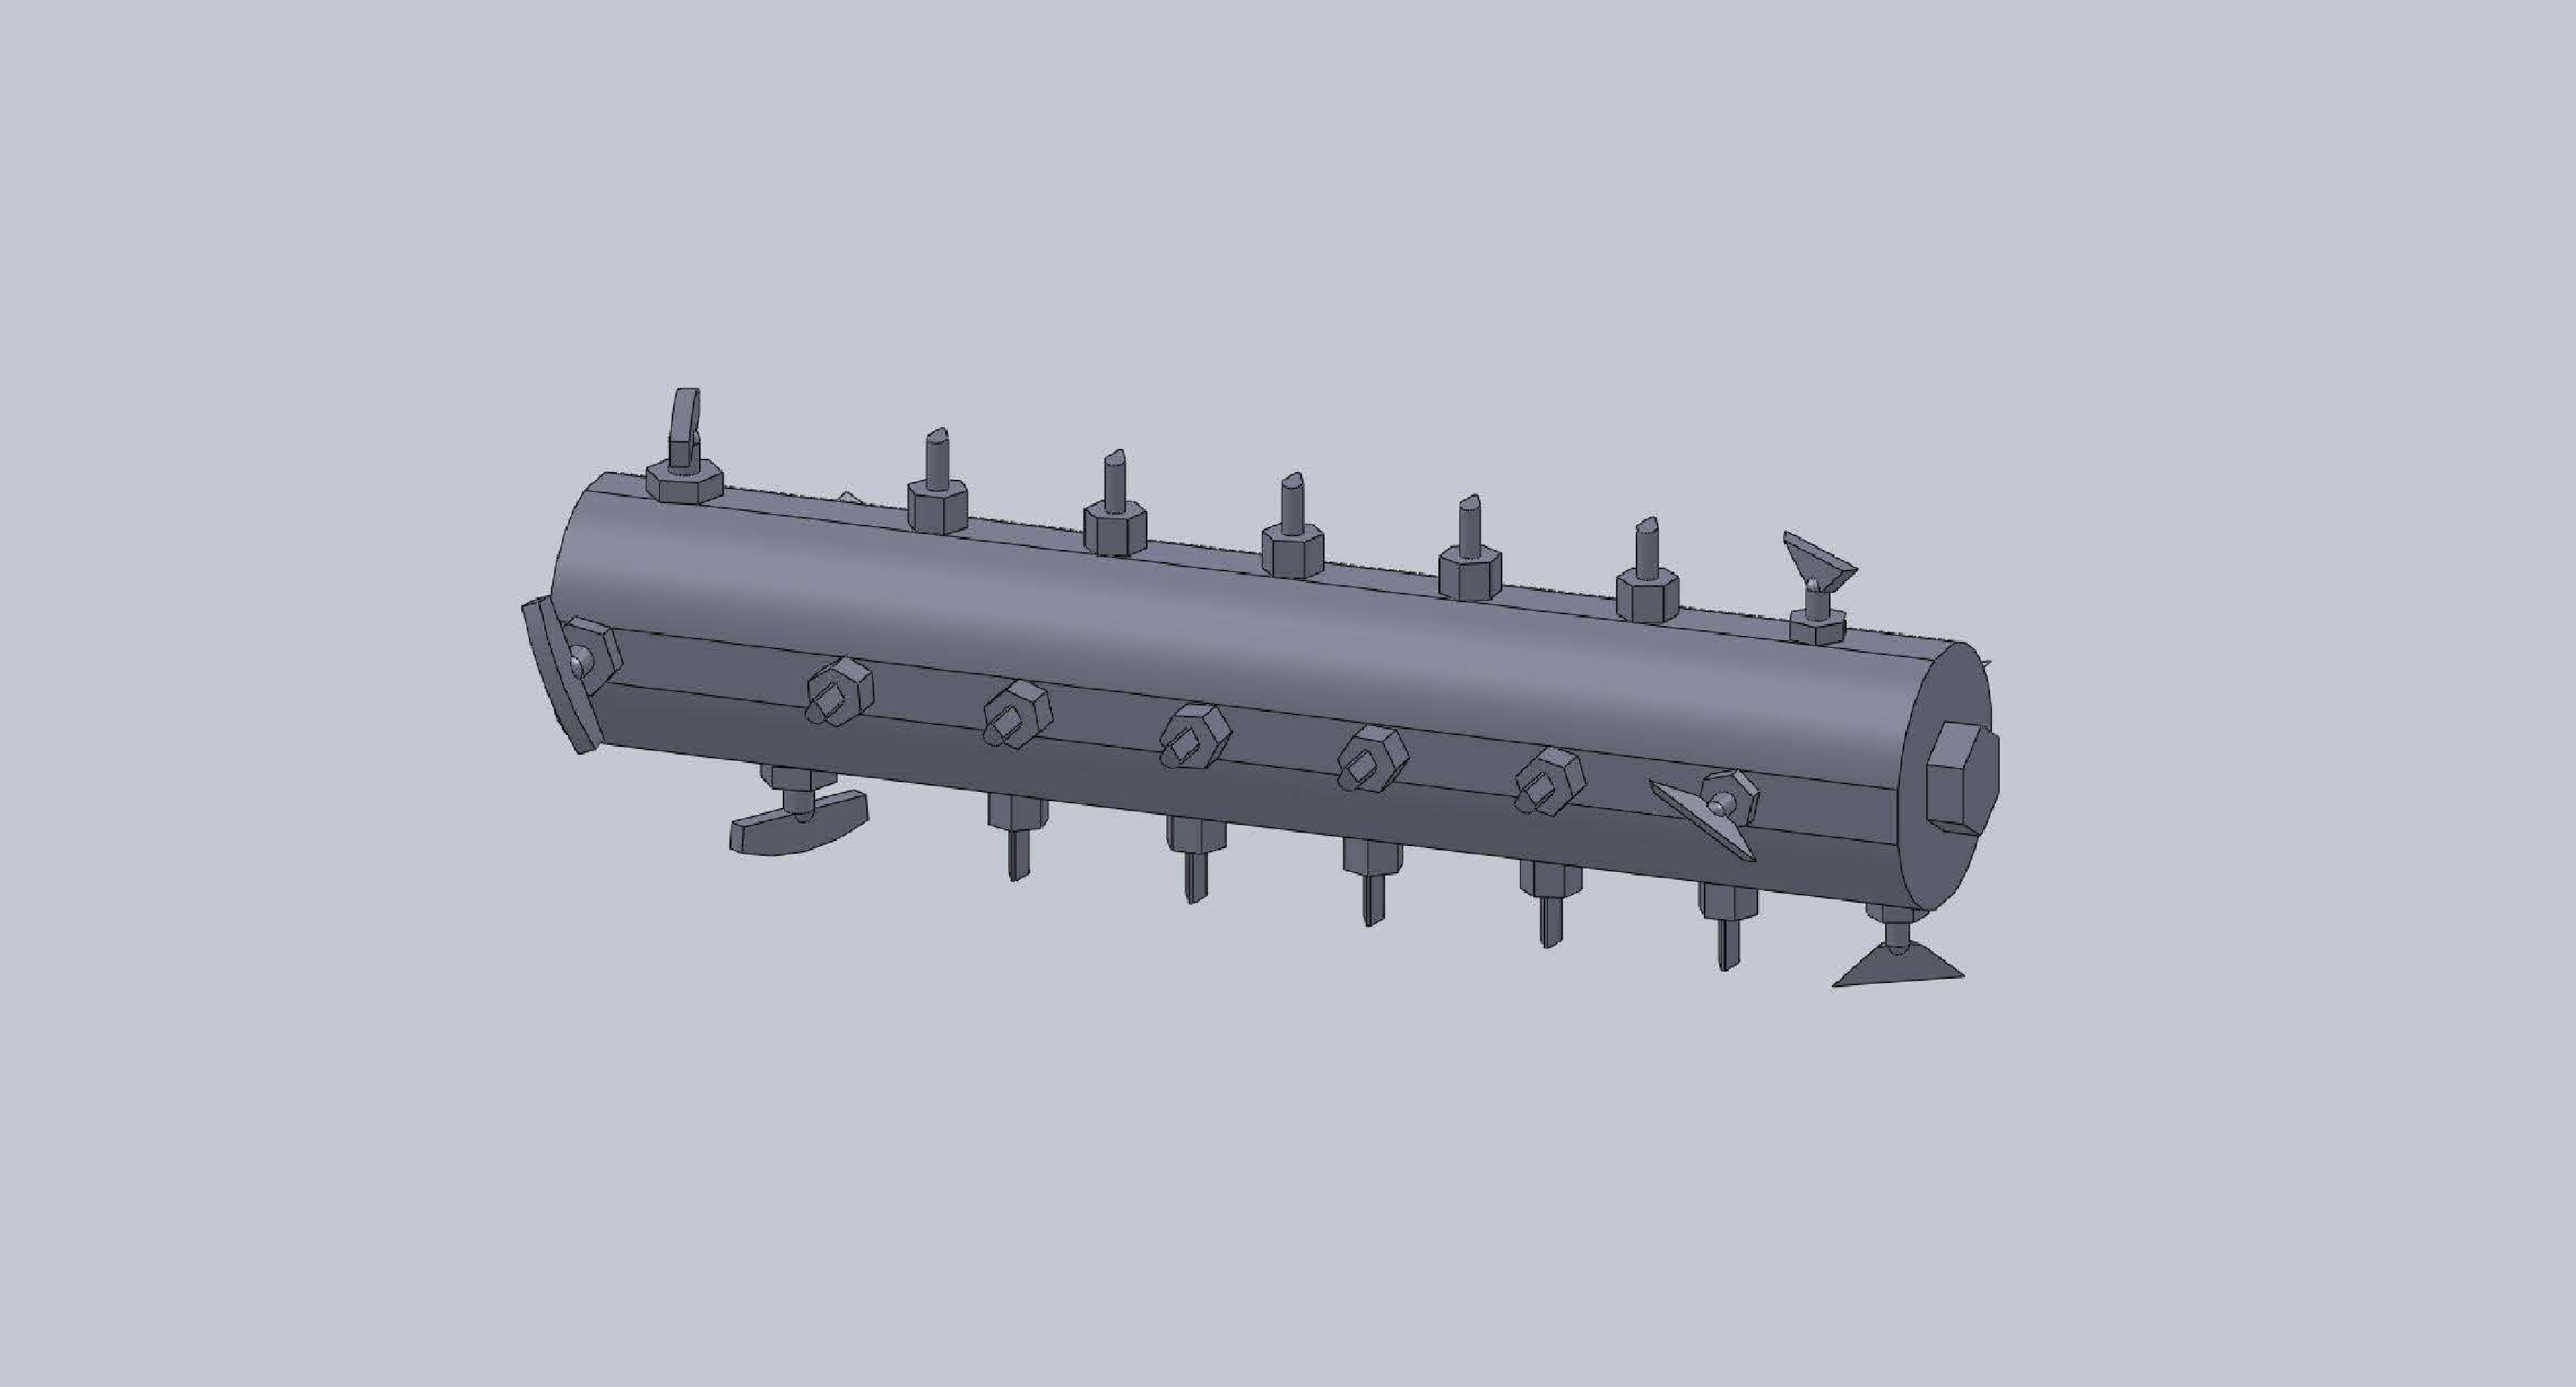
\includegraphics[scale=0.2]{impeller_final_pic.pdf}
	      \caption{a) Shows the side view of the impeller. b) and c) show the front and back views of the impeller which correspond to the inlet and outlet ends respectively.}
	      %\caption{hello yuk}
	      \label{fig:mthds_dem_charles_impeller}
	      \end{figure}    
	    
	      \begin{figure}[H]
			
	      \begin{subfigure}{.3\textwidth}
  			\centering
  			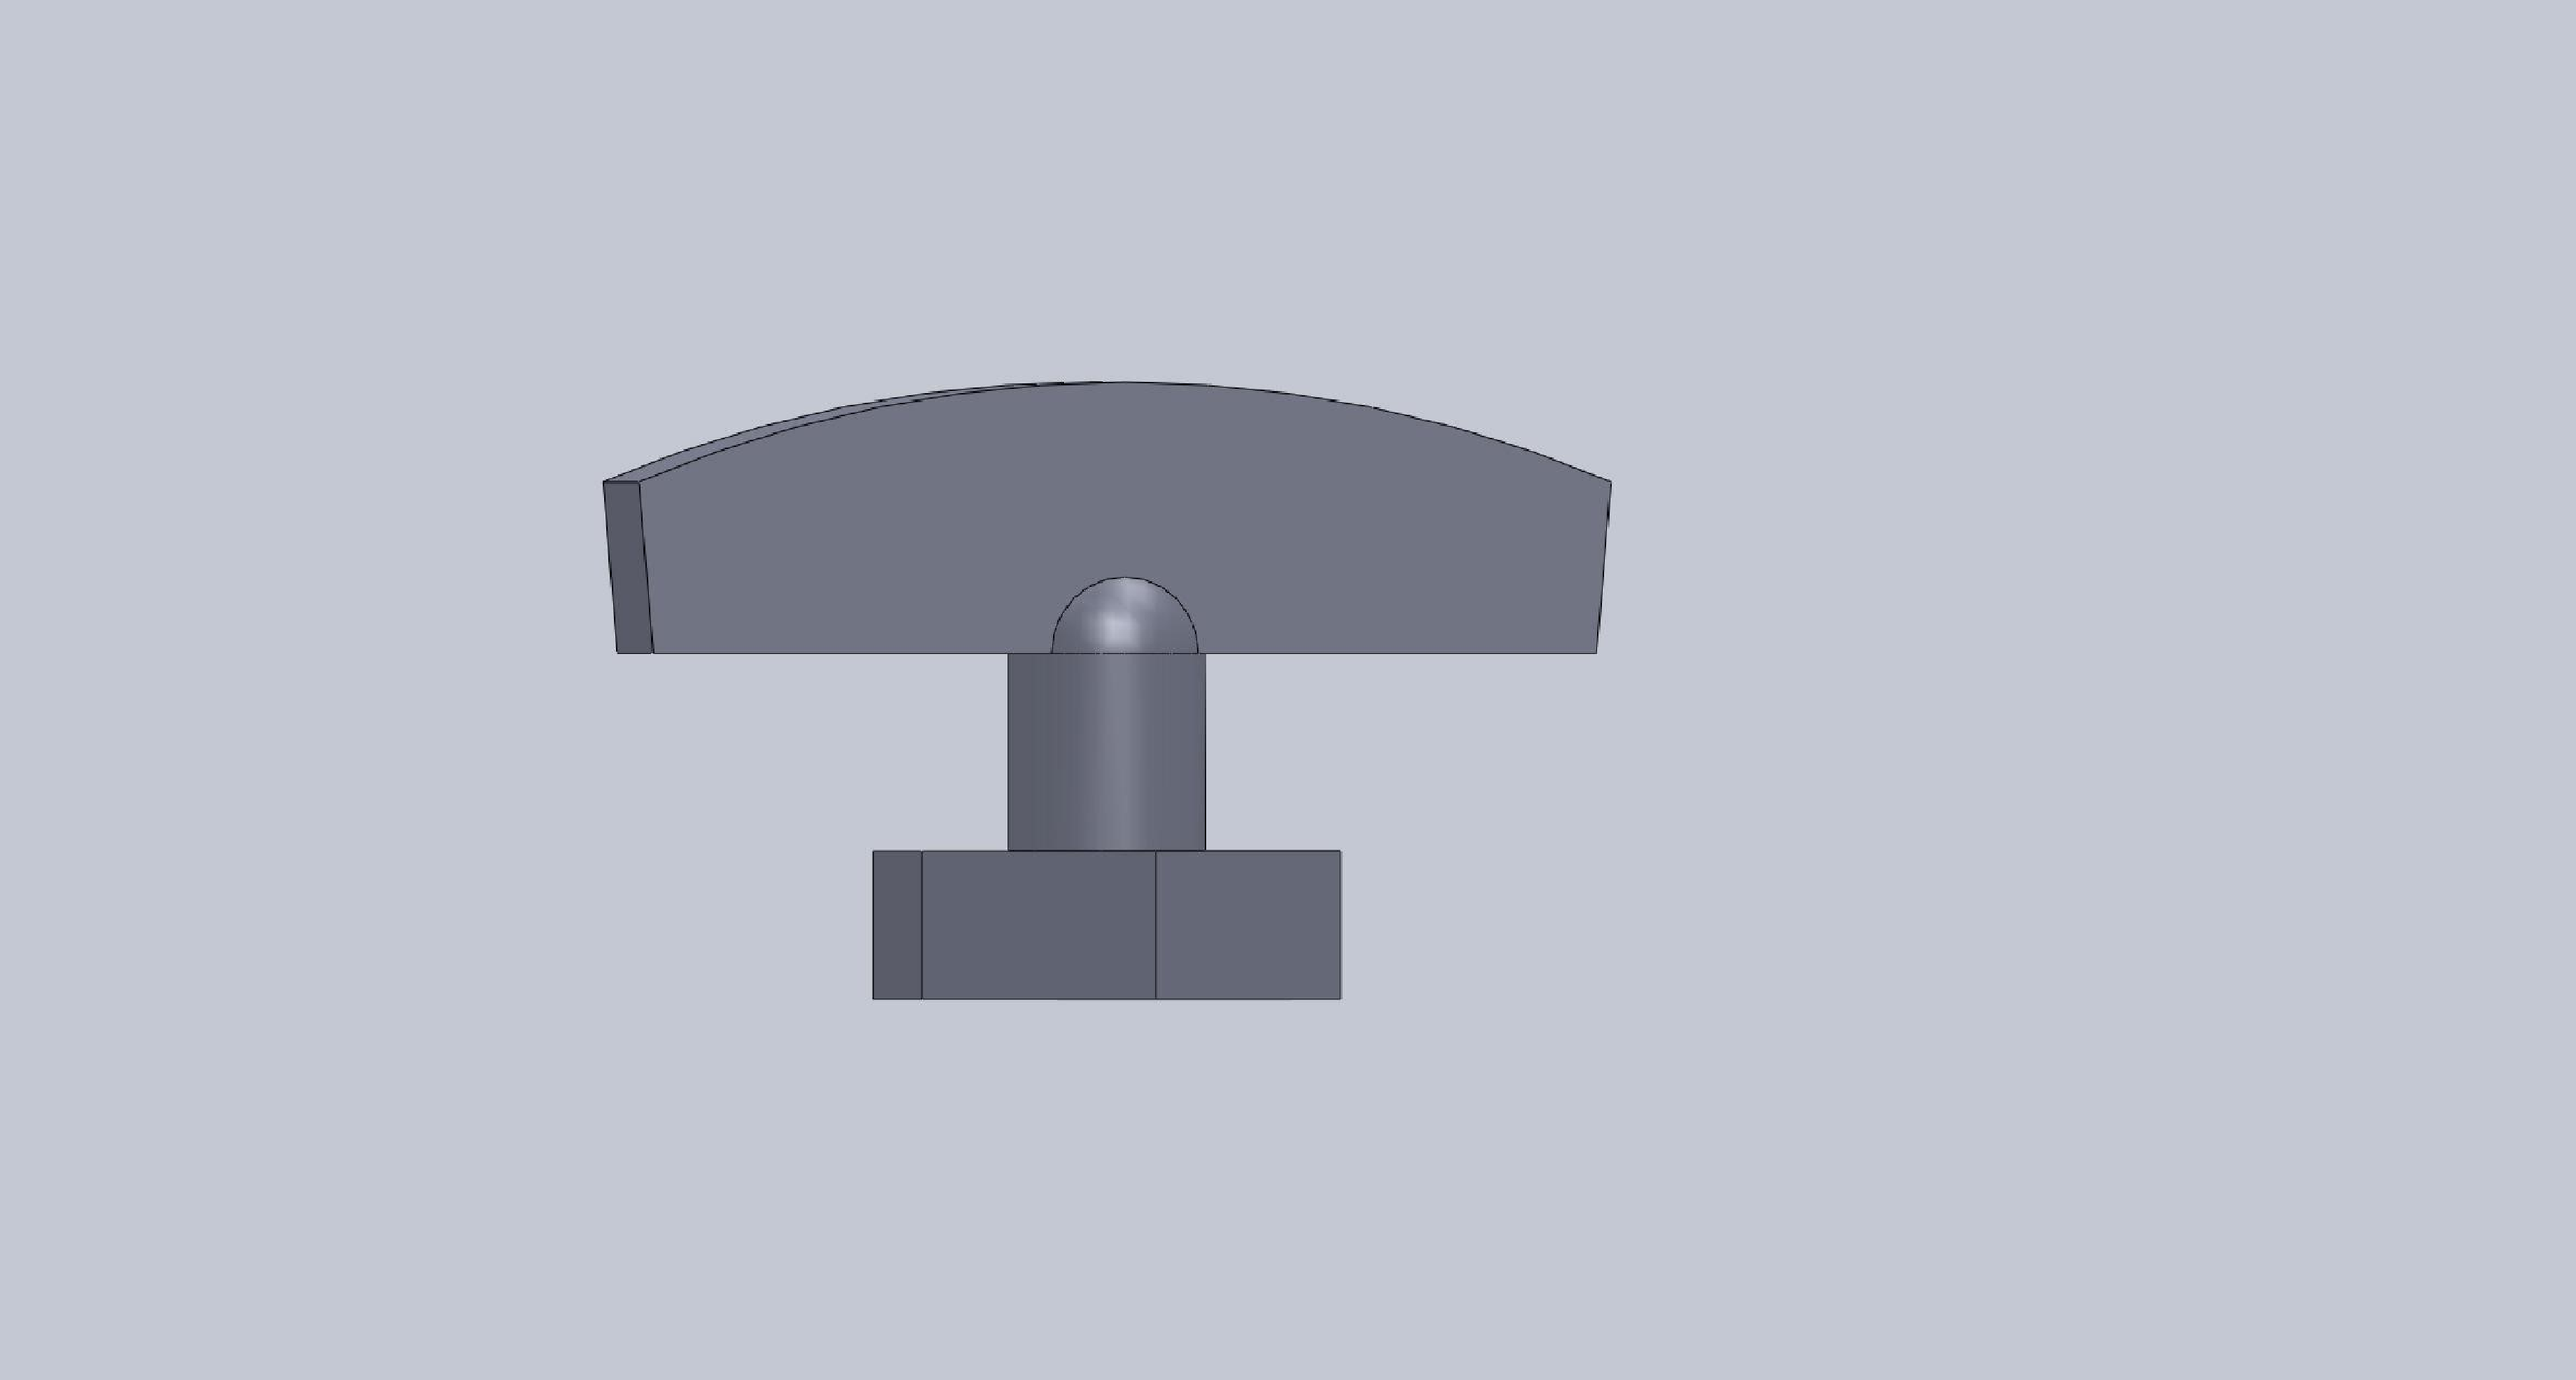
\includegraphics[scale=0.075]{feed_element.pdf}	      
  			\caption{Feed element}
  			\label{fig:mthds_dem_feed_element}
			\end{subfigure}%
			\begin{subfigure}{.3\textwidth}
  			\centering
			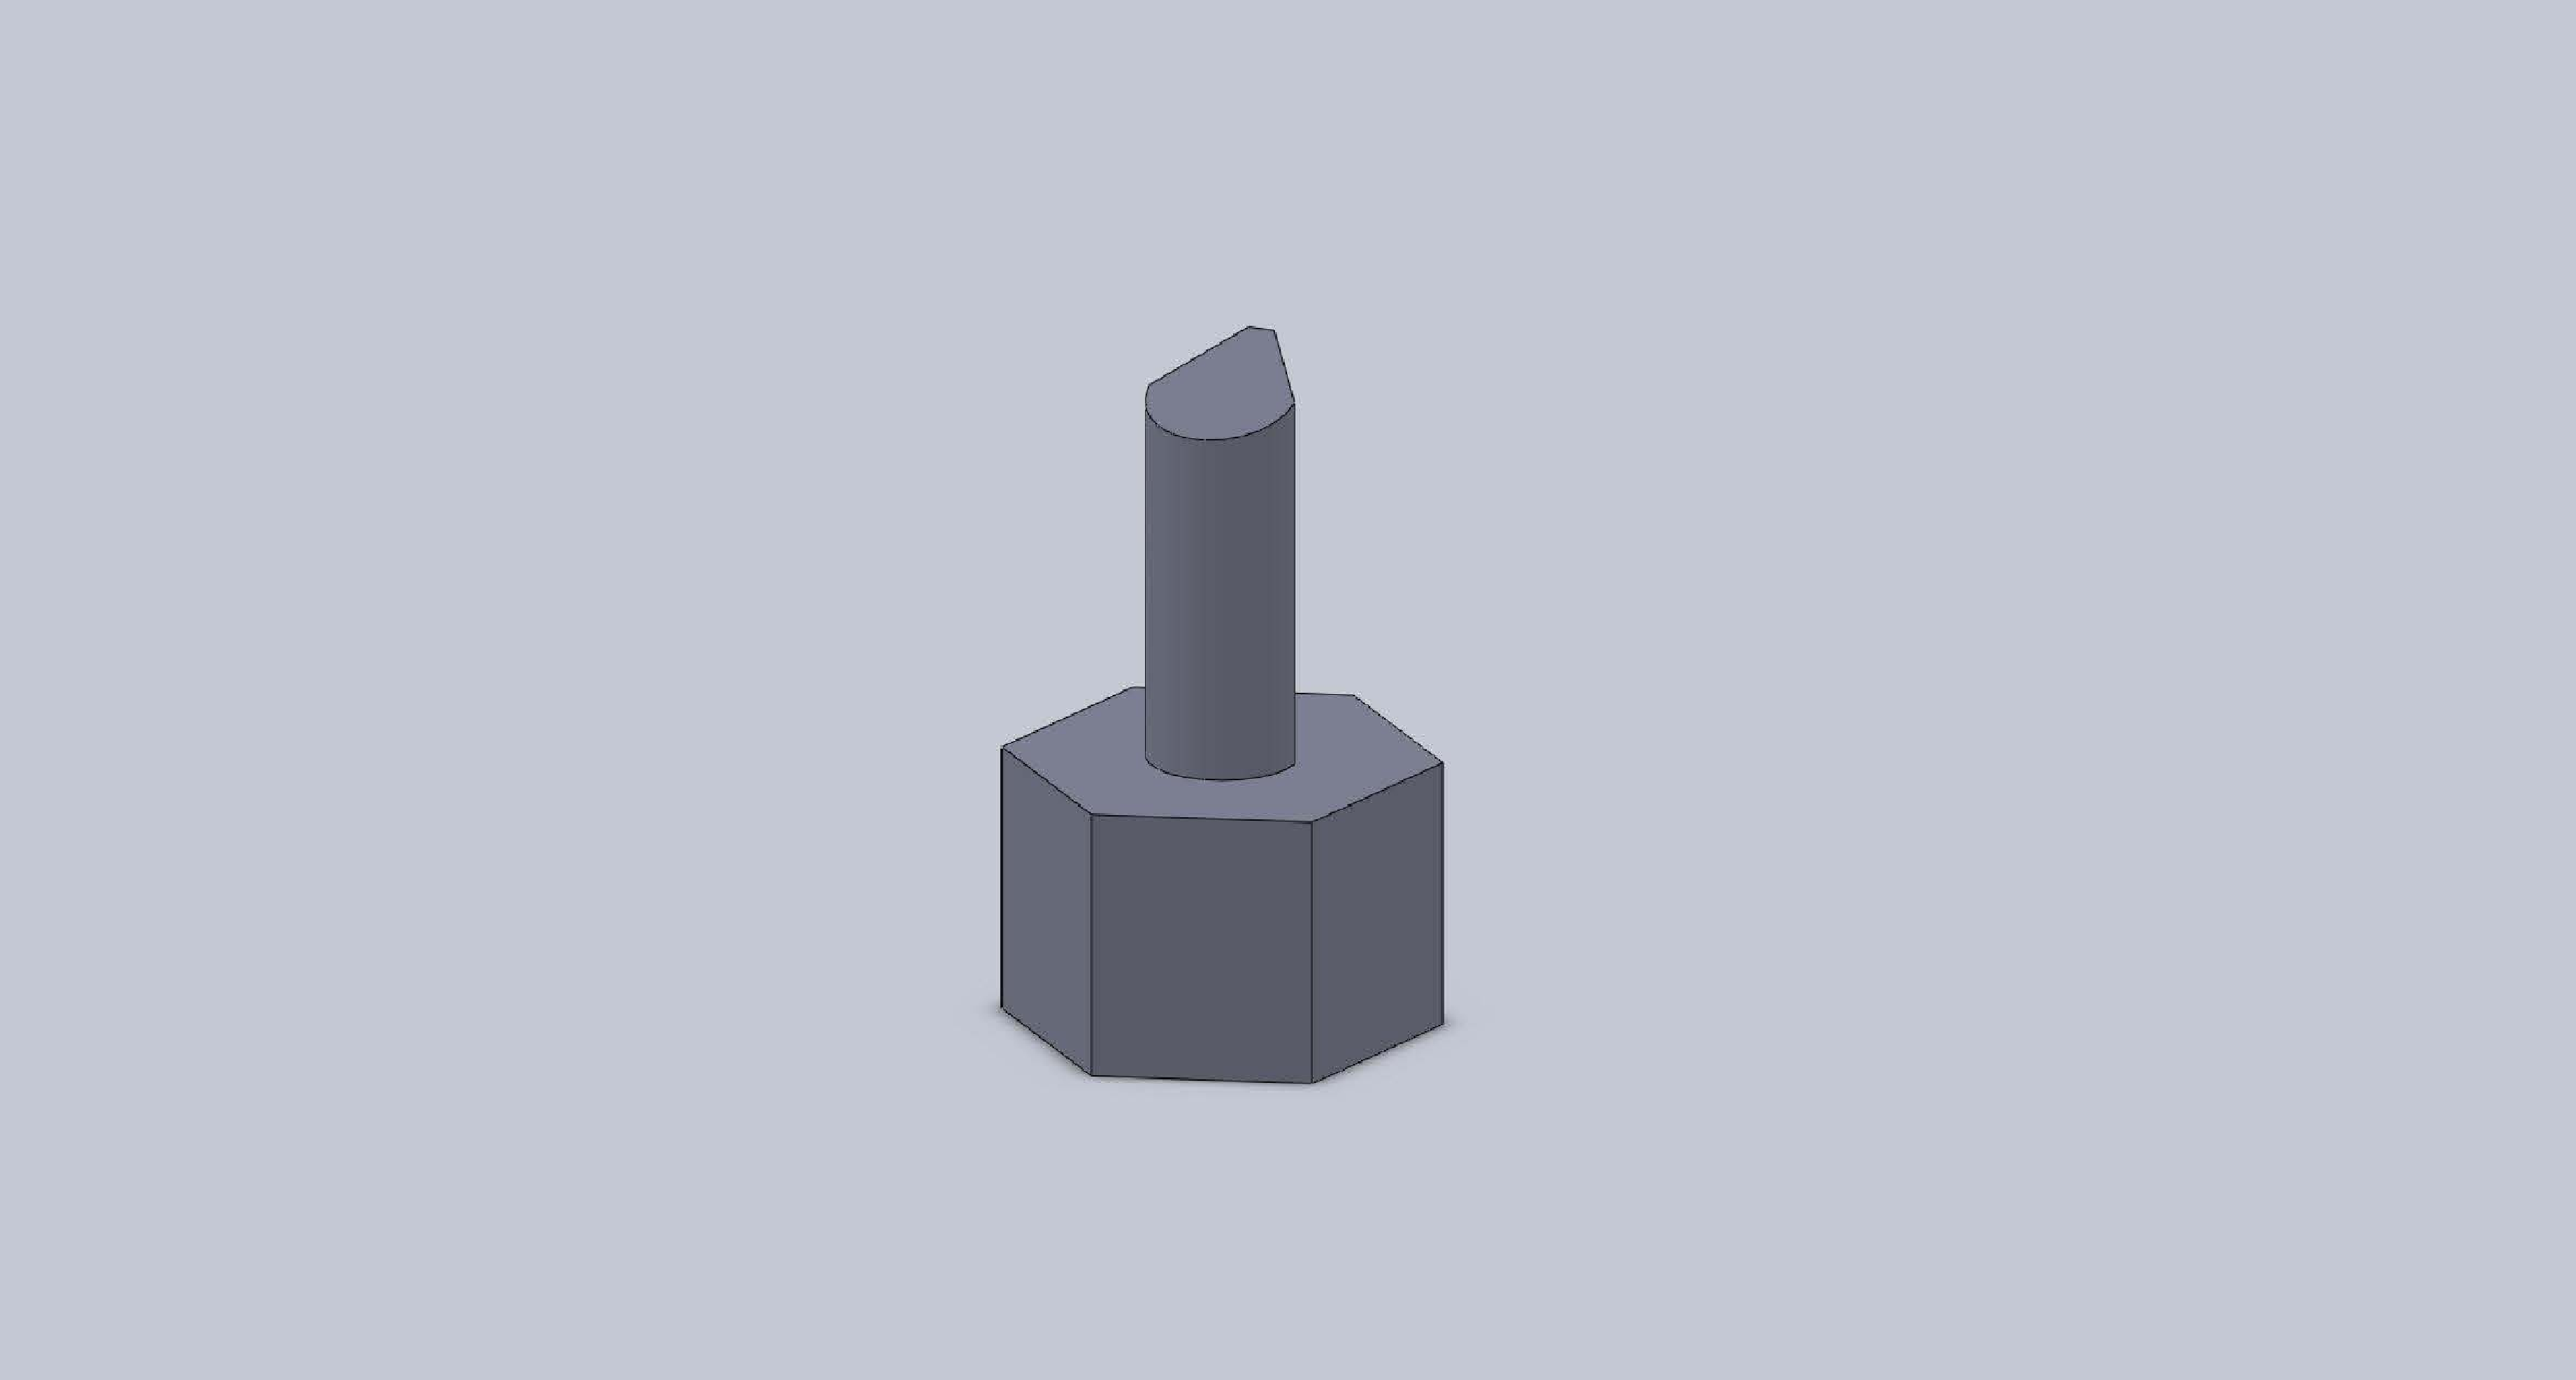
\includegraphics[scale=0.075]{shear_element.pdf}
  			\caption{Shear element}
  			\label{fig:mthds_dem_shear_element}
			\end{subfigure}
	      	\begin{subfigure}{.3\textwidth}
  			\centering
	      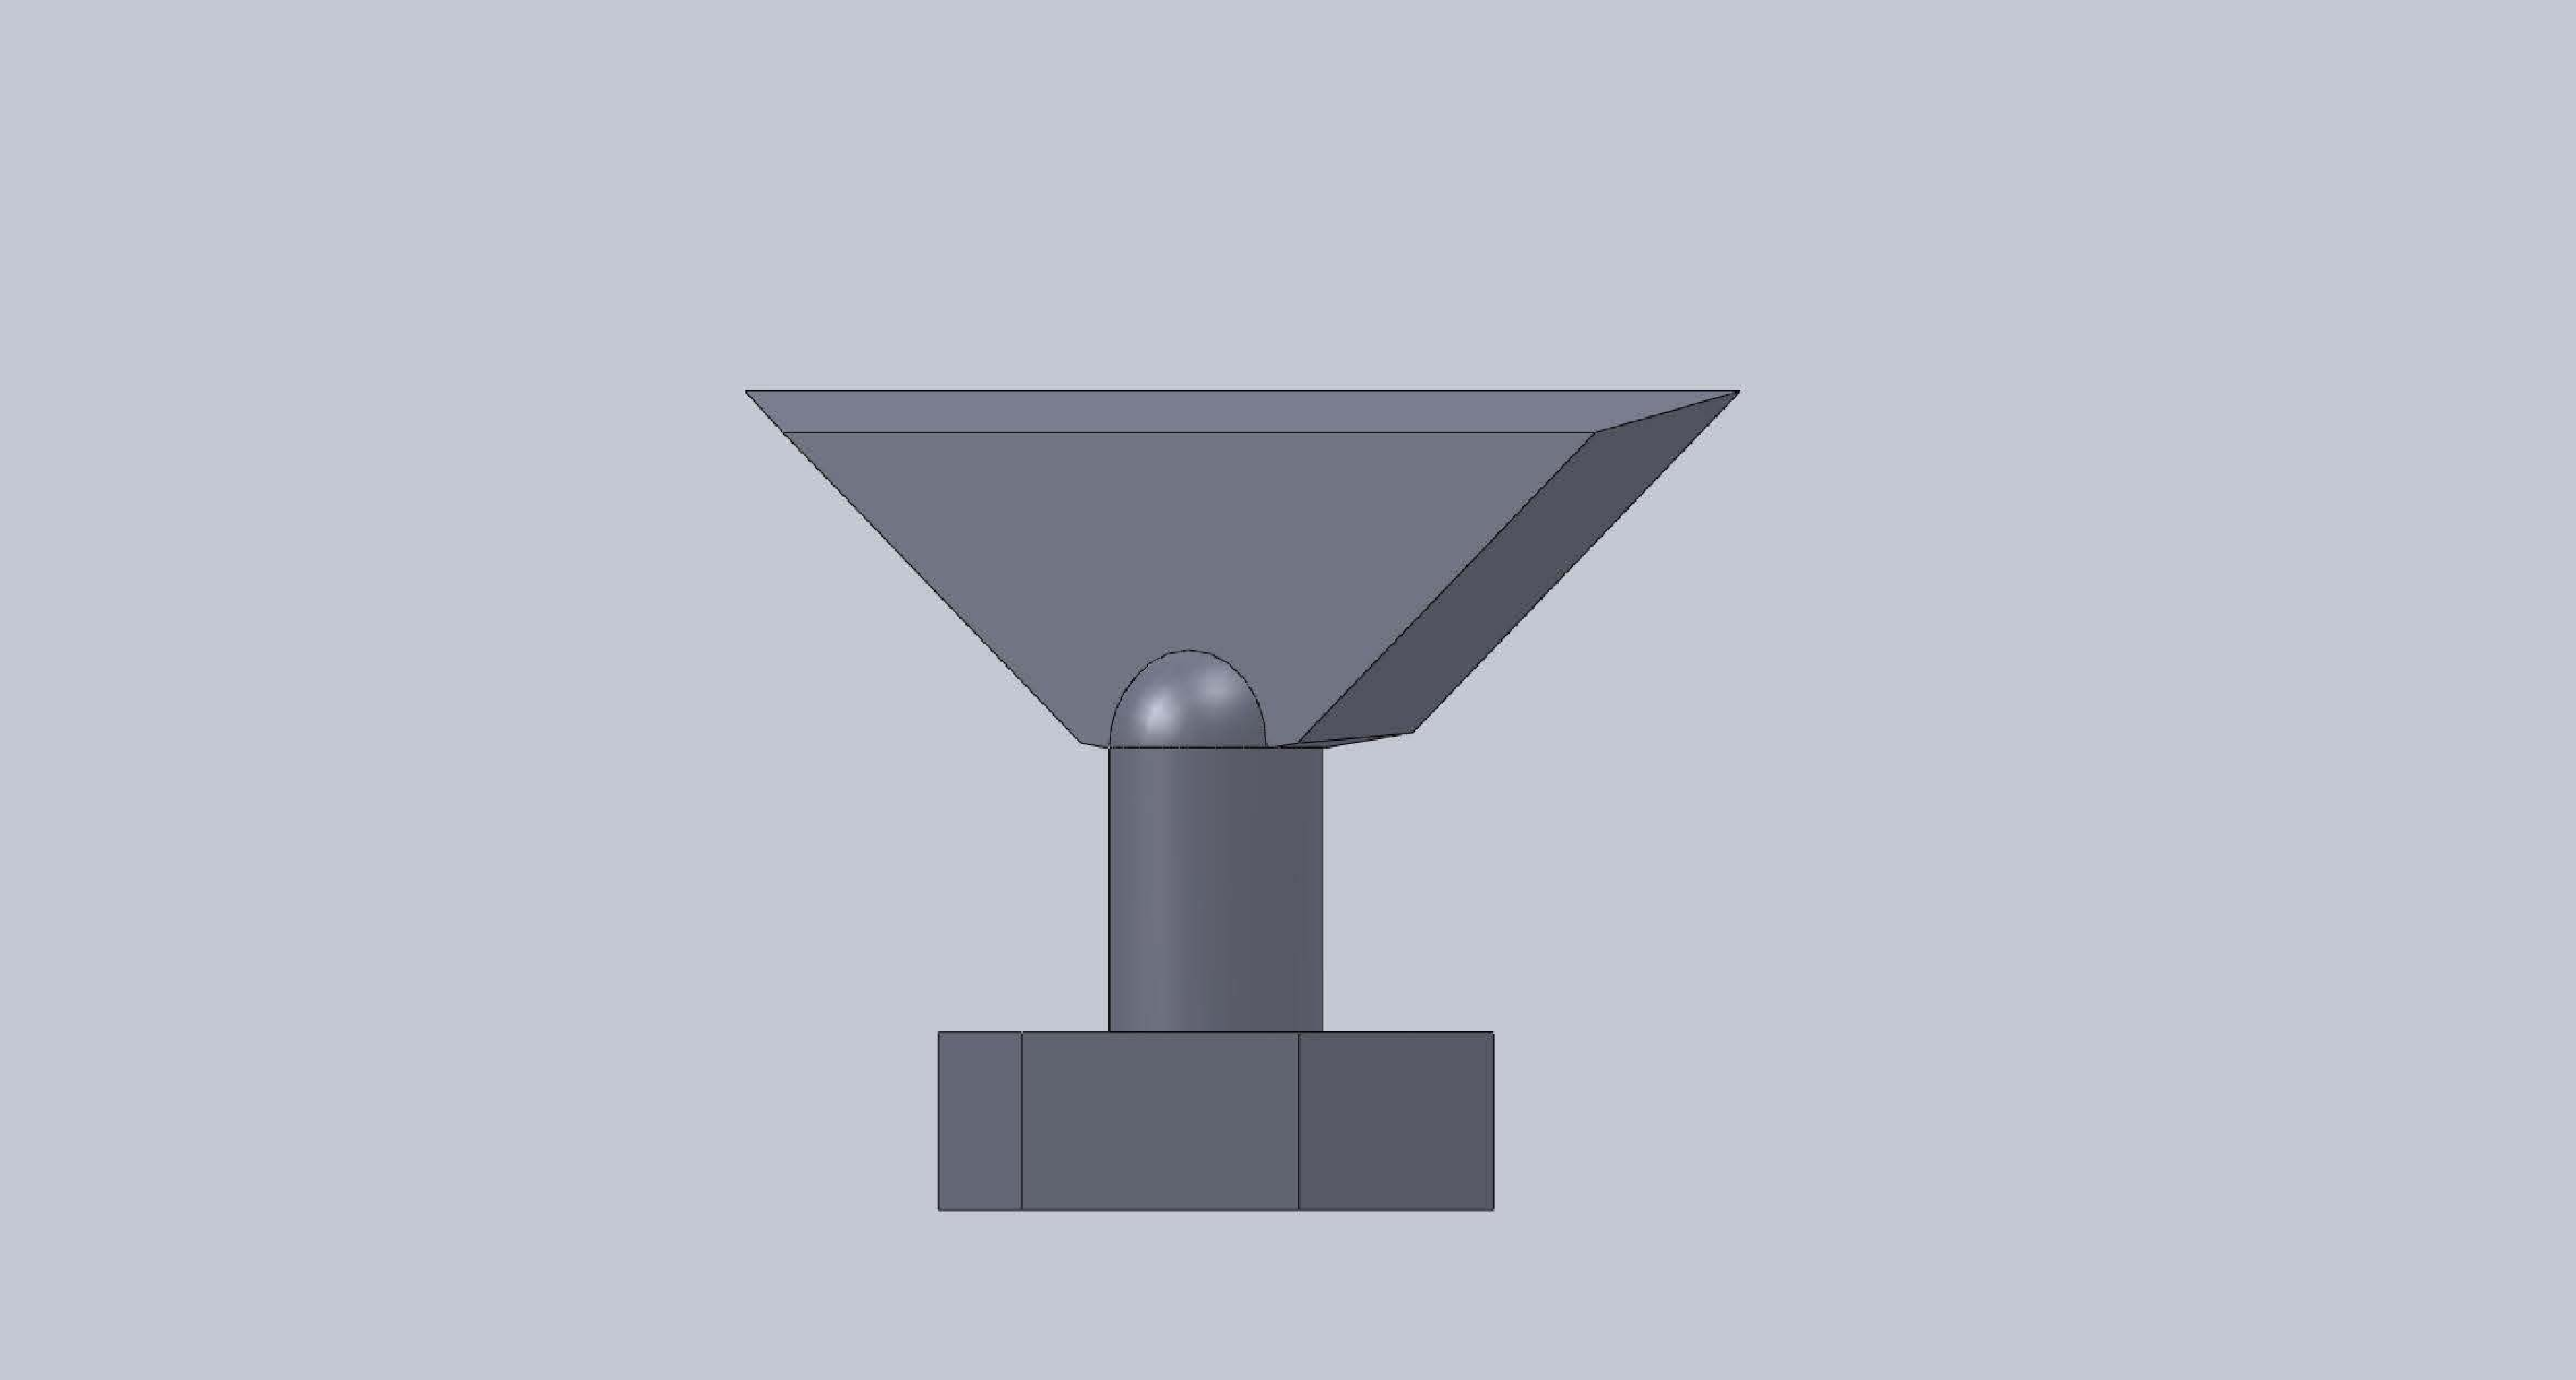
\includegraphics[scale=0.075]{exit_element.pdf}
  			\caption{Exit element}
  			\label{fig:mthds_dem_exit_element}
			\end{subfigure}
	      


	      \caption{ Various components of the impeller}
	      %\caption{hello tesh}
	      \label{fig:mthds_dem_charles_fig5pt3and4_blades_n_isometric}
	      \end{figure}     
	    
	
	    
	
	    \subsubsection{Meshing}
	    \par After the geometry was built in SolidWorks$^{TM}$ (Dassault Syst\`{e}mes) the shell and impeller were exported as STL files. The coarsest output option was used to keep the STL files small and simple for faster computations times. They were also exported not keeping there original coordinates  This resulted in the impeller having 2802 faces and 1281 points with approximately a file size of 775 KBs. The shell had 1948 faces and 720 points and size was about 544 KBs.  
	    \par Meshlab was used to align the STL files for importing into LIGGGHTS\textsuperscript{\textregistered}. No mesh treatments were used on the STLs. 
	    \par The meshes were then imported into LIGGGHTS\textsuperscript{\textregistered} using the write command. This resulted in 50 elements of the impeller file having "highly skewed elements", which have more than 5 neighbours per surface or have an angle less than 0.0181185 degrees, that according to LIGGGHTS\textsuperscript{\textregistered} would degrade parallel performance. The write exclusion list command in LIGGGHTS\textsuperscript{\textregistered} was used and this exclusion list file as then used in the simulation to skip the highly skewed elements during the simulation 
	    %The shell did not have any skewed elements \textcolor{cyan}{(FUTURE SOLUTION? - perhaps we can use the output from liggghts exclusion list to find exact elements of issue. then we can use meshlab to exclude those peices or remesh thos individual pieces into better shapes with less skewed elements. might be better for a letter paper though}
	    
	    \subsubsection{DEM input file settings}
	    \par The DEM simulation in LIGGGHTS\textsuperscript{\textregistered} are setup using an input script which defines the physical parameters of the particles, importing of the geometry, particle insertion commands, various physics models to be used during the simulation as well as various compute and dump commands to help print the data required for post-processing of the data. A script was prepared each of the particle was considered granular in nature. The Hertzian model was used for non-adhesive elastic contact between the granular particles. The particles were inserted inside the granluator from the inlet at a constant mass flow rate of 15 kilgrams per hour. The rotation speed of the impeller was kept throughout the study at 2000 rotations per minute. Such a high rotation speed was chosens since this would lead to high shear between the particles and the walls of the shell resulting in better size control of the granules. There were 2 sets of simulations that were performed, one with mono-sized partcles and second consisting of a distribution of sizes. The particle radii chosen for mono-sized simulation varied 0.59mm - 2mm, consecutive particles radii had volume twice of one before them. The radii range of the distributed size simulation was 1mm - 3mm. The difference in the mechanics of these two simulations is dicussed later in the results section. The physical constants used for the simulations are given in Table \ref{table:mthds_dem_input}.
	    \par The simulation data was collected after a constant number of iterations for the visulation of the particles inside the shell, further post processing and to be used in the PBM. The collisions between each of the particles and the collisions between of the particle and the geometry was also collected. 

	    	\begin{table}[!htb]%[H]
	\caption{Physical Properties of the particle for the LIGGGHTS\textsuperscript{\textregistered} input script} \label{table:mthds_dem_input}
	\begin{center}
	\begin{tabular}{l|c|c}
	\hline
	\bf{Parameter} &\bf{Value} &\bf{Units}\\
	\hline
	Young's Modulus of particles  & $8 \times 10^{6}$ & $N.m^{-2}$\\
	Young's Modulus of Geometry  & $1 \times 10^{9}$ & $N.m^{-2}$\\
	Poisson's Ratio & $0.2$ & $-$\\
	Coefficient of restitution (constant for all collisions) & $0.4$ & $-$\\
	Coefficient of static friction & $0.5$ & $-$\\
	Coefficient of rolling friction  & $0.2$ & $-$\\
	Density of the granules & $500$ & $kg.m^{-3}$\\
	\hline
	\end{tabular}
	\end{center}
	\end{table}

	    \subsubsection{DEM data post processing}
	    \par The post processing of the data obtained from the DEM simulations was done using MATLAB\textsuperscript{\textregistered}. The first test run on the output data was to determine if the simulation had reached steady-state. The mass inside the granulator was found out by averaging it over 5 time steps and then compared to mass inside the granulator after every 10000 time steps (about $5$x$10^{-4}$ seconds) with a tolerance of about 10\%. If the mass was found to be constant for most of the iterations, it was considered to be at steady state. Another test to determine steady state was to monitor the number of collision inside the granulator. It can be seen that the number of collision start to oscillate around a mean value. The number of collisions were then plotted and steady state time was determined. 
	    \par A precautionary script was also run so as to determine that no particles were lost due to overlap of the geometry with the particles as well as from particle particle overlap.
	     
	    
	  \subsection{PBM}
	    \subsubsection{Model Development}
	    \par The main PBM equation developed for this work can be expressed as shown below:
	    \begin{align}
	    \frac{d}{dt}F(s_1,s_2,x)=\Re_{agg}(s_1,s_2,x)+R_{break}(s_1,s_2,x)+\dot{F}_{in}(s_1,s_2,x)-\dot{F}_{out}(s_1,s_2,x)
	    \label{eqn:mthds_pbm_overall} 
	    \end{align}
%	    \par \textcolor{red}{citation?}    
	    
	    \par where, $F(s_1,s_2,x)$ is the number of particles with an API volume of $s_1$ and an excipient volume of $s_2$ in the spatial compartment $x$. The rate of change of number of particles with time in different size classes depend on the rate of aggregation $\Re_{agg}(s_1,s_2,x)$ and the rate of breakage $\Re_{break}(s_1,s_2,x)$. Also, the rate of particles coming into, $F_{in}(s_1,s_2,x)$ and going out, $F_{out}(s_1,s_2,x)$ of the spatial compartment due to particle transfer affect the number of particles in different size classes. 
	The rate of change of liquid volume is calculated using the equation: 
	
	    \begin{align}
	    \frac{d}{dt}F(s_1,s_2,x)l(s_1,s_2,x)=& \Re_{liq,agg}(s_1,s_2,x)+\Re_{liq,break}(s_1,s_2,x)+\dot{F}_{in}(s_1,s_2,x)l_{in}(s_1,s_2,x)\notag\\
	    &-\dot{F}_{out}(s_1,s_2,x)l_{out}(s_1,s_2,x)+F(s_1,s_2,x)\dot{l}_{add}(s_1,s_2,x)
	    \end{align}
	    
	    \par where, $l(s_1,s_2,x)$ is the amount of liquid volume in each particle with API volume of $s_1$ and excipient volume of $s_2$ in the spatial compartment $x$. $\Re_{liq,agg}(s_1,s_2,x)$ and $\Re_{liq,break}(s_1,s_2,x)$ are respectively the rates of liquid transferred between size classed due to aggregation and breakage. $l_{in}(s_1,s_2,x)$ and $l_{out}(s_1,s_2,x)$ are respectively the liquid volumes of the particles coming in and going out of the spatial compartment. $l_{add}(s_1,s_2,x)$ is the volume of liquid acquired by each particle in the compartment at every time step due to external liquid addition. 
	    \par Similarly, the rate of change of gas volume is calculated using the following equation: 
	    \begin{align}
	    \frac{d}{dt}F(s_1,s_2,x)g(s_1,s_2,x)=& \Re_{gas,agg}(s_1,s_2,x)+\Re_{gas,break}(s_1,s_2,x)+\dot{F}_{in}(s_1,s_2,x)g_{in}(s_1,s_2,x)\notag\\
	    &-\dot{F}_{out}(s_1,s_2,x)g_{out}(s_1,s_2,x)+F(s_1,s_2,x)\dot{g}_{cons}(s_1,s_2,x)
	    \end{align}
%	    \par \textcolor{red}{citation?}
	    
	    \par where, $g(s_1,s_2,x)$ is the gas volume of each particle with API volume of $s_1$ and excipient volume of $s_2$ in the spatial compartment $x$. $\Re_{gas,agg}(s_1,s_2,x)$ and $\Re_{gas,break}(s_1,s_2,x)$ are respectively the rates of gas transferred between size classed due to aggregation and breakage. $g_{in}(s_1,s_2,x)$ and $g_{out}(s_1,s_2,x)$ are respectively the gas volume of the particles entering and leaving the spatial compartment. $g_{cons}(s_1,s_2,x)$ is the volume of gas coming out of each particle in the compartment at every time-step due to consolidation of the particles. 
	    \par The rate of aggregation, $\Re_{agg}(s_1,s_2,x)$ in Equation \ref{eqn:mthds_pbm_overall} is calculated as  
	     \begin{align}
	     \Re_{agg}(s_1,s_2,x)=& \frac{1}{2}\int _0^{s_1} \int_0^{s_2} \beta(s_1',s_2',s_1-s_1',s_2-s_2',x)F(s_1',s_2',x)F(s_1-s_1',s_2-s_2',x)ds_1'ds_2'\notag\\ 
	     &- F(s_1,s_2,x)\int _0^{s_{max_1}-s_1} \int_0^{s_{max_2}-s_2} \beta(s_1,s_2,s_1',s_2',x)F(s_1',s_2',x)ds_1'ds_2'
	     \end{align}
%	     \par \textcolor{red}{citation?}
	     
	    \par where, the aggregation kernel, $\beta(s_1,s_2, s_1',s_2',x)$ is expressed as a function of collision frequency ($C$) and collision efficiency ($\psi$) –
	    \begin{align}
	    \beta(s_1,s_2,s_1',s_2',x) = & \beta_oC(s_1,s_2,s_1',s_2')\psi(s_1,s_2,s_1',s_2',x)
	    %\beta(s_1,s_2,s_1',s_2',x) = & \beta_o*(V(s_1,s_2,x)+V(s_1',s_2',x))^{\gamma}*(c(s_1,s_2,x)\notag\\
	    %&+c(s_1',s_2',x))^{\alpha}\left(1-\frac{(c(s_1,s_2,x)+c(s_1',s_2',x))^{\delta}}{2}\right)^{\alpha}
	    \label{eqn:mthds_pbm_beta_kernal}
	    \end{align}
	    %\par \textcolor{red}{citation?}
	    
	    where, $\beta_o$ is aggregation rate constant.
	    \par Collision frequency is a function of particle size and is calculated from the number of collisions between group of particles obtained from LIGGGHTS\textsuperscript{\textregistered}. A recent study shows that collision frequency depends on PSD as well (\cite{sen2014}). Collision frerquency can be expressed as:
	    \begin{align}
	    C(s_1,s_2,s_1',s_2')=\frac{N_{coll}(s_1,s_2,s_1',s_2')}{F(s_1,s_2)F(s_1',s_2')\Delta t}
	    \label{eqn:collfreq}
	    \end{align}
	    \par In equation(\ref{eqn:collfreq}), $N_{coll}$ is the number of collision between two solid particles in time interval $\Delta t$. The $\psi$ in equation (\ref{eqn:mthds_pbm_beta_kernal}) can be expressed asvi 
	    
	    \begin{align}
	    \psi((s_1,s_2,s_1',s_2') = 
	    \left\{\begin{matrix}
	    \psi_0,\hspace{0.2cm} LC((s_1,s_2) \geq LC_{min}\hspace{0.2cm} or\hspace{0.2cm} LC((s_1',s_2') \geq LC_{min}	\\ 
	    0,\hspace{0.2cm} LC((s_1,s_2) < LC_{min}\hspace{0.2cm} or\hspace{0.2cm} LC((s_1',s_2') < LC_{min}
	    \end{matrix}\right.
	    \end{align}
	    \par In above equation, $LC$ is the liquid content of particles and $LC_{min}$ stands for minimum liquid content required for coalescence of particle.  
	    \par Similarly, the breakage rate is expressed as-
	
	    \begin{align}
	    \Re_{break}(s_1,s_2,x) = \int_0^{s_{max_1}} \int_0^{s_{max_2}} K_{break}(s_1',s_2',x)F(s_1',s_2',x)ds_1'ds_2' - K_{break}(s_1,s_2,x)F(s_1,s_2,x)
	    \end{align}
%	    \par \textcolor{red}{citation?}
	    
	    \par where, the breakage kernel $K_{break}(s_1,s_2,x)$ is formulated as – 
	    
	    \begin{align}
	    K_{break}(s_1,s_2,x) = C_{impact}\int_{U_{break}}^{\infty}p(U)dU
	    %K_{break}(s_1,s_2,x)=\left(\frac{4}{15\pi}\right)^{(\frac{1}{2})}G_{shear}exp\left(-\frac{B}{R(s_1,s_2,x)}\right)
	    \end{align}
%	    \par \textcolor{red}{citation?}
	
	      %\par where, $G_{shear}$ is the shear rate exerted by the impeller on the granules. $R(s_1,s_2,x)$ is the radius of the granule that breaks and $B$ is the breakage kernel constant. $G_shear$ is calculated as $\frac{\nu_{impeller}*D_{impeller}*PI}{60}$ where $\nu_{impeller}$ and $D_{impeller}$ are respectively the rotational speed and diameter of the impeller.
	      \par The rate of increase of liquid volume of one particle, $\dot{l}_{add}(s_1,s_2,x)$ is expressed as $\frac{(s_1+s_2)(\dot{m}_{spray}(1-c_{binder})-\dot{m}_evap)}{m_{solid}(x)}$ where, $(s_1+s_2)$  is the total solid volume of the particle; $\dot{m}_spray$ is the rate of external liquid addition, $c_{binder}$ is the concentration of binder in the external liquid (which is assumed to be zero in this case as pure liquid is added); $\dot{m}_{evap}$ is the rate of evaporation of liquid from the system (which is also assumed to be zero in this case) and $m_{solid}$ is the total amount of solid present in the compartment.
	      \par The rate of decrease in gas volume per particle due to consolidation is calculated using the following expression: 
	      
	      \begin{align}
	      \dot{g}_{cons}(s_1,s_2,x)=c*(\nu_{impeller})^{\omega}*V(s_1,s_2,x)\frac{(1-\epsilon_{min})}{s} [g(s_1,s_2,x)+l(s_1,s_2,x) -(s_1+s_2)\frac{\epsilon_{min}}{1-\epsilon_{min}}]
	      \end{align}          
	    
	    \par where, $c$ and $\omega$ are the consolidation constants; $v_{impeller}$ is the impeller rotational speed; $V(s_1,s_2,x)$ is the volume of particle, $\epsilon_{min}$ is the minimum porosity; $g(s_1,s_2,x)$ and $l(s_1,s_2,x)$ are respectively the gas and liquid volume of the particle.
	  
	    \par Particle transfer rate, $F_{out}(s_1,s_2,x)$ in Equation \ref{eqn:mthds_pbm_overall} is calculated as $F(s_1,s_2,x)*\frac{\nu_{compartment(x)}*dt}{d_{compartment}}$ where, $\nu_{compartment(x)}$ and $d_{compartment}$ are respectively the average velocity of particles in compartment $x$ and the distance between the mid-points of two adjacent compartment, which is the distance particles have to travel to move to the next spatial compartment. $dt$ is the time-step.
	The values of various parameters used in the model are provided in Table \ref{table:mthds_pbm_parameters}.
	
	\begin{table}[!htb]
	\caption{Parameters for PBM from Anik's hetero. agg. paper. currently place holder} \label{table:mthds_pbm_parameters}
	\begin{center}
	\begin{tabular}{l|c|c|c}
	\hline
	\bf{Parameter} &\bf{Symbol} &\bf{Value} &\bf{Units}\\
	\hline
	Time step & $\delta t$ & $0.5$ & $s$\\
	Total granulation time & $T$ & $45, 45$ & $s$\\
	Velocity in axial direction & $v_{axial}$ & $1$ & $ms^{-1}$\\
	Velocity in radial direction & $v_{radial}$ & $1$ & $ms^{-1}$\\
	Aggregation constant & $\beta_0$ & $1\times10^{-9}$ & $-$\\
	Initial particle diameter & $R$ & $150$ & $\mu m$\\
	Breakage kernel constant & $B$ & $0$ & $-$\\
	Diameter of impeller & $D$ & $0.114$ & $m$ \\
	Impeller rotation speed & $RPM$ & $2000$ & $rmp$\\
	Minimum granule porosity & $\epsilon_{min}$ & $0.2$ & $-$\\
	Consolidation rate & $C$ & $0$ & $-$\\
	Total starting particles in batch & $F_{initial}$ & $1 \times 10^{6}$ & $-$\\
	Liquid to solid ratio & $L/S$ & $0.35$ & $-$ \\
	Number of Compartments & $c$ & $4$ & $-$ \\
	Number of first solid bins & $s$ & $16$ & $-$\\
	Number of second solid bins & $ss$ & $16$ & $-$\\
	\hline
	\end{tabular}
	\end{center}
	\end{table}
	
	    \subsubsection{Parameters}
	    
	    
	  \subsection{PBM Parallel C++}
	    \subsubsection{Discretization \& Parallelizing PBM}
	    \par The PBM was discretized by converting each of its coordinates in to discrete bins. For the spatial coordinates a linear bin spacing was used. For the internal coordinates, solid,liquid, and gas a nonlinear binning was used. %\textcolor{cyan}{get more details from Anik on this will probably need more detail on binning for reproducability}
	    \par Once the PBM had been discretized (compartmentalized/binned) a finite differences method was used which created a system of ordinary differential equations (ODEs). The numerical integration technique used to evaluate the system of ODEs was first order Euler integration as it is commonly used to solve these types of systems and author  found it improved speeds while having minimal impact on accuracy. To obtain the most optimal parallel performance, when solving the PBM, work loads were distributed in a manner which took into account the shared memory and distributed memory aspects of the clusters the PBM was being run on. To parallelize the model in a why which could take advantage of shared memory but still effectively run across a distributed system both OMP and MPI were implemented. 
	    \par One MPI process was used per CPU socket and one OMP process was used per CPU core, as authors (\cite{Bettencourt2017}) found it resulted in the best performance. MPI was used for message passing from one node to another while OMP was used for calculations on each node that could be efficiently solved using a shared memory system %\textcolor{cyan}{i.e. calculations were inter-dependent but could be computed simultaneously.} 
	    \par Pseudo code is presented below illustrating how the calculations are distributed and carried out during the simulation. For each time step the MPI processes are made responsible for a specific chunk of the spatial compartments. Then each OMP thread, inside of each MPI process, is allocated to one of the cores of the the multi-core CPU the MPI process is bound too. The OMP processes divide up and compute $\Re_{agg}$ and $\Re_{brk}$. %(\textcolor{cyan}{include more detail about how they do it? last paper reviewer complained that could not understand figure by JUST reading what I wrote about it in meat of paper}) 
	    \par After $\Re_{agg}$ and $\Re_{brk}$ are calculated the MPI processes calculate the new PSD value for their chunk at that specific time step, $F_{t,c}$. The slave processes send their $F_{t,c}$ to the master processes which collects them into the complete $F_{t,all}$. The master process then broadcasts the $F_{t,all}$ value to all slave processes. 	
	    \par A crucial feature of the PBM is that the current PSD ($F_{t,all}$) value is used to compute a new time step size for the next iteration. This means all of the MPI processes need to have the same dynamic time step size at each iteration for the calculations to be properly carried out in parallel. Since the completely updated $F_{t,all}$ value is shared before calculating a new time step each process will have the same $F_{t,all}$ value. As a result each process calculates the same size for the new time step. 
	%\textcolor{cyan}{ Did not include the liquid and gas PBMs in this but hoping they will be some what assumed? Also the Ragg omp distributed work is an a}
	%\textcolor{red}{what about private OMP vars specified that has impact on how model is solved etc. Should look into this. might change based on locking/blocking tests that need to be implemented still.}   
	
	  \begin{algorithm}[!h]
	   \caption*{\bf{Algorithm: }Pseudo code}
	    \begin{algorithmic}[*]
	     \While{ $t<t_{final}$ }
	      \par // the spatial domain is divided into equal chunks (with in 1 bin size)
	      \par // each MPI process is assigned on chunk of spatial domain shown as $c_{low}$ to $c_{up}$ 
	      \par // sum all $c_{low_i}$ to $c_{up_i}$ is = to [0,numCompartments]
	  
	        \For{each MPI processes} $c = c_{low_i}$ to $c_{up_i}$
		  	\par   // each MPI process is further divided with OMP to take advantage of multi-core CPU
			\par   // each OMP process is allocated to a single compute core
			\par   // $\Re$ integrals $(i1)$ $\int_{0}^{s_2}$, $(i2)$ $\int_{0}^{s_{max_2}-s_2}$, and $(i3)$ $\int_{0}^{s_{max_2}-s_2}$ are divided into smaller integrals
			\par  // $\int_{i_1low_n}^{i_1up_n}$, $\int_{i_2low_n}^{i_2up_n}$, and $\int_{i_3low_n}^{i_3up_n}$ which are solved by the "n" OMP processes
	        \par   // allocated to that MPI process (CPU)
	          \For{ each OMP process}
	
	     \begin{align}
	     \Re_{agg}(s_1,s_2,c)=& \frac{1}{2}\int_{0}^{s_{1}} \int_{i_1low_n}^{i_1up_n} \beta(s_1',s_2',s_1-s_1',s_2-s_2',c)F(s_1',s_2',c)F(s_1-s_1',s_2-s_2',c)ds_1'ds_2'\notag\\ 
	     &- F(s_1,s_2,c)\int _{0}^{s_{max_1}-s_1} \int_{i_2low_n}^{i_2up_n} \beta(s_1,s_2,s_1',s_2',c)F(s_1',s_2',c)ds_1'ds_2'\notag
	     \end{align}
	     \begin{align*}
	    \Re_{break}(s_1,s_2,c) = \int_{0}^{s_{max_1}} \int_{i_3low_n}^{i_3up_n} K_{break}(s_1',s_2',c)F(s_1',s_2',c)ds_1'ds_2' - K_{break}(s_1,s_2,c)F(s_1,s_2,c)
	     \end{align*}
	         \EndFor 
	     \begin{align*}
	   F_{t,c} &= \frac{\Delta F(s_1,s_2,c)}{\Delta t}\Delta t  + F(s_1,s_2,c)_{t-1}\\
	                  &=   (\Re_{agg}(s_1,s_2,c)+\Re_{break}(s_1,s_2,c)+\dot{F}_{in}(s_1,s_2,c)-\dot{F}_{out}(s_1,s_2,c))\Delta t + F(s_1,s_2,c)_{t-1}
	     \end{align*}
	
	        \EndFor
	     \State MPI Send $F_{t,c}$ to Master MPI process
	     \State MPI Recv $F_{t,c}$ from MPI all slave processes
	     \State Master consolidate all $F_{t,c}$ chunks into a complete $F_{t,all}$
	     \State Master does inter-bin particle transfers (updates $F_{t,all}$)
	     \State MPI Bcast $F_{t,all}$ to all slave processes
	     \State $t_{new} = t + timestep$
	        
	     \EndWhile   
	
	\end{algorithmic}
	\end{algorithm}   
	    
	  
	  \subsection{RP \& PBM+DEM Communication}
	

A primary challenge faced is the scalable execution of multiple (often two,
but possibly more) heterogeneous simulations that need to run independently
but have a need to communicate and exchange information. Traditionally each
simulation is submitted as an individual job, but that brings invariably leads
to the situation where each simulations gets through the batch-queue systems
independent of the other. So although the first-through-the-queue is ready to
run, it stalls fairly soon waiting for the other simulation to make it through
the queue.  On the other hand MPI capabilities can used to  execute both
simulations as part of a single multi-node job.  Thus whereas the former
method suffers from unpredictable queue time for each job, the latter is
suitable to execute tasks that are homogeneous and have no dependencies, and
relies on the fault tolerance of MPI which are inadequate.


The Pilot abstraction~\cite{review_pilotreview} solves these issues:  The
pilot abstraction, (i) uses a container-job as a placeholder to acquire
resources via the local resource management system (LRMS) and,  (ii) to
decouple the initial resource acquisition from task-to-resource assignment.
Once the pilot (container-job) is scheduled via the LRMS, it can then directly
be populated with the computational tasks. This functionality allows all the
computational tasks to be executed directly on the resources, without being
queued at the LRMS individually. This approach thus supports the requirements
of task-level parallelism and high-throughput as needed by science drivers.

RADICAL-Pilot is an implementation of the pilot abstraction, engineered to
support scalable and efficient launching of heterogeneous tasks
across different platforms.

	
	  
	\section{Results}
	  \subsection{PBM}
	    \subsubsection{PBM Validation}
	      
	
	      \begin{figure}[H]
	      \centering
	      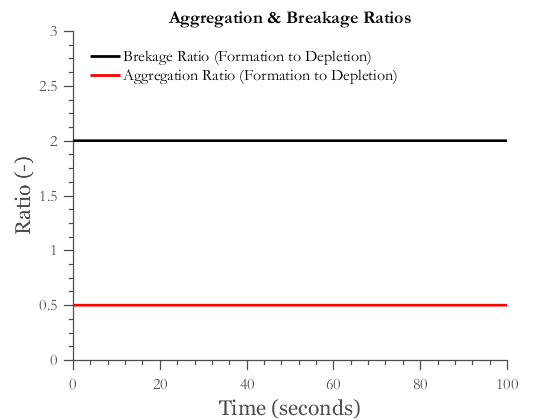
\includegraphics[scale=0.5]{rslts_anik_pbm_ratios}
	      \caption{Ratio of formation-to-depletion through aggregation and breakage over time. Breakage ratio of 2 and aggregation ratio of 0.5 indicate mass conservation in the model. \textcolor{red}{NOTE DID NOT HAVE .fig file for this figure so it is in as JPG will need to replace} }
	      %\caption{hello tesh}
	      \label{fig:rslts_anik_pbm_ratios}
	      \end{figure}
	     
	     \par The ratio between the number of particles formed due to aggregation and the number of particles depleted due to aggregation and the ratio of the number of particles formed due to breakage to the number of particles depleted due to breakage are plotted. In aggregation two particles agglomerate to form one particle and in breakage one particle breaks to form two particles. So, these ratios are expected to be 0.5 and 2 respectively. As can be seen from Figure \ref{fig:rslts_anik_pbm_ratios}, these ratios are accurate confirming that mass is conserved accurately in the model.
	\par The granulator was divided into 3 compartments spatially and the total volume, solid volume and pore volume and the median diameter $d_50$ in each compartment were plotted to study the granulation behaviour and are shown in Figure \ref{fig:rslts_anik_pbm_total_vol_solid_pore_d50}. 
	\par It can be seen from Figure \ref{fig:rslts_anik_pbm_total_vol} that the total volume starts to increase first in compartment 1 followed by compartment 2 and then compartment 3. This happens as gradually particles entering compartment 1 moves to the other compartment due to particle transfer from compartment 1 to compartment 2 and then compartment 3. In Figure \ref{fig:rslts_anik_pbm_total_solid_vol} it is observed that the solid volume similar to the total volume increases first in compartment 1 and last in compartment 3. The solid volume becomes constant and equal in all the compartments at around 30-50 seconds and steady state is reached when the rate of particle volume being transported through the compartments and leaving the system is equal to the rate of particles entering the system. Although, as seen in Figure \ref{fig:rslts_anik_pbm_total_pore_vol} the pore volume which is the sum of the gas and the liquid volume is highest in compartment 3 and lowest in compartment 1. This happens due to the external liquid addition to the system. As the particles move from compartment 1 to compartment 3, they gradually acquire a higher amount liquid, thereby increasing the pore volume. In Figure \ref{fig:rslts_anik_pbm_d50}, the $D_50$ is seen to be increasing from compartment 1 to 3. This happens because of the size enlargement of large particles coming in from the previous compartment because of the external liquid added to each compartment and a longer residence time in the granulator. 
	
	\begin{figure}[H]
	    \centering
	    \begin{subfigure}[b]{0.45\textwidth}
	        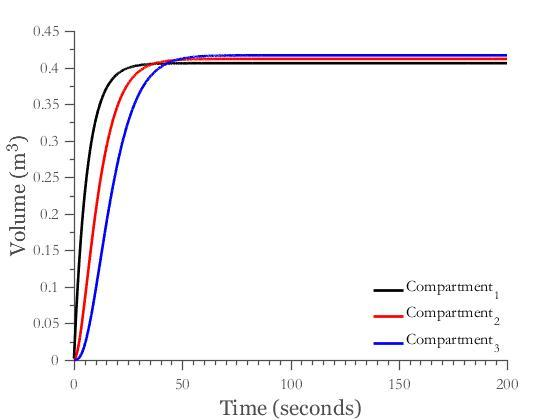
\includegraphics[width=\textwidth]{rslts_anik_pbm_total_vol}
	        \caption{Total volume in all compartments}
	        \label{fig:rslts_anik_pbm_total_vol}
	    \end{subfigure}
	    ~ %add desired spacing between images, e. g. ~, \quad, \qquad, \hfill etc. 
	      %(or a blank line to force the subfigure onto a new line)
	    \begin{subfigure}[b]{0.45\textwidth} 
	        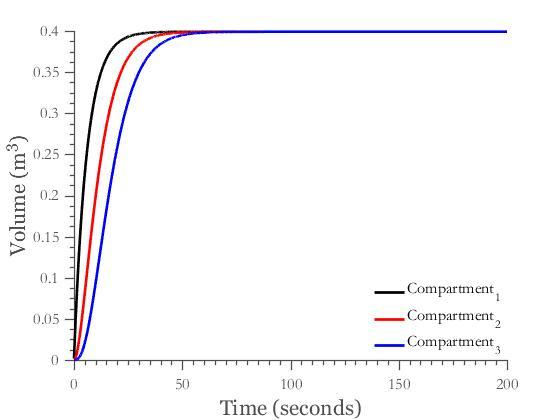
\includegraphics[width=\textwidth]{rslts_anik_pbm_total_solid_vol}
	        \caption{Total solid volume in all compartments}
	        \label{fig:rslts_anik_pbm_total_solid_vol}
	    \end{subfigure}
	    ~ %add desired spacing between images, e. g. ~, \quad, \qquad, \hfill etc. 
	    %(or a blank line to force the subfigure onto a new line)
	    
	    \begin{subfigure}[b]{0.45\textwidth}
	        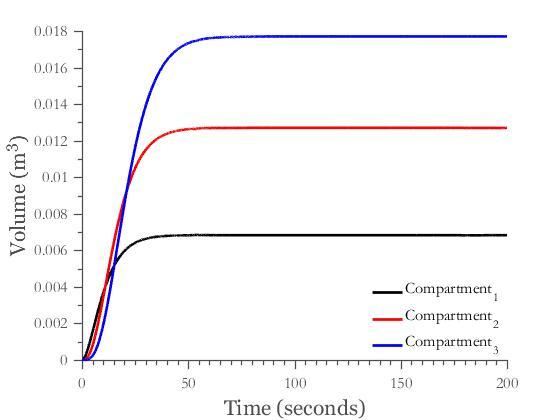
\includegraphics[width=\textwidth]{rslts_anik_pbm_total_pore_vol}
	        \caption{Total pore volume in all compartments}
	        \label{fig:rslts_anik_pbm_total_pore_vol}
	    \end{subfigure}
	    \begin{subfigure}[b]{0.45\textwidth}
	        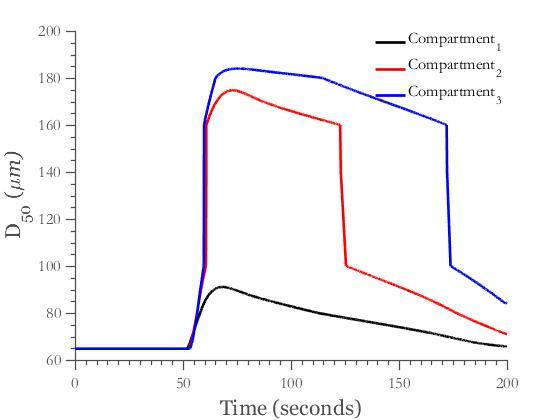
\includegraphics[width=\textwidth]{rslts_anik_pbm_d50}
	        \caption{D$_{50}$ in all compartments}
	        \label{fig:rslts_anik_pbm_d50}
	    \end{subfigure}
	
	    \caption{Volume and D50 in all compartments over time. Volumes become constant as steady state is reached. Median diameter increases and then decreases as bigger particles leave the system and smaller particles occupy that volume.}\label{fig:rslts_anik_pbm_total_vol_solid_pore_d50}
	\end{figure}
	
	
	    \subsubsection{Parallel C++ PBM Validation}
	   \par show PSD or $D_50$ is the same as Matlab or serial PBM
	   \par 1. fig $D_50$ Matlab vs Parallel
	      \begin{figure}[!htb]
	      \centering
	      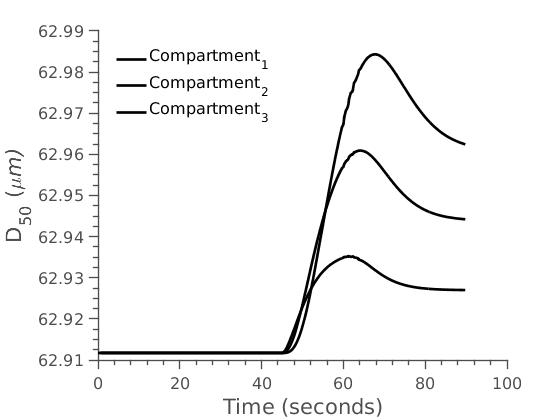
\includegraphics[scale=0.5]{rslts_pbm_d_50_pll_vldtn}
	      \caption{ $D_{50}$ of Matlab PBM vs Parallel PBM}
	      %\caption{hello tesh}
	      \label{fig:rslts_pbm_d_50_vldtn}
	      \end{figure}
	    
	    \subsubsection{Parallel PBM Performance}
	     \par show that RP has minimal impact on performance 
	    \par show that performance is mostly unaffected by RP 
	    \par 1. fig scaling 
	      \begin{figure}[H]
	      \centering
	      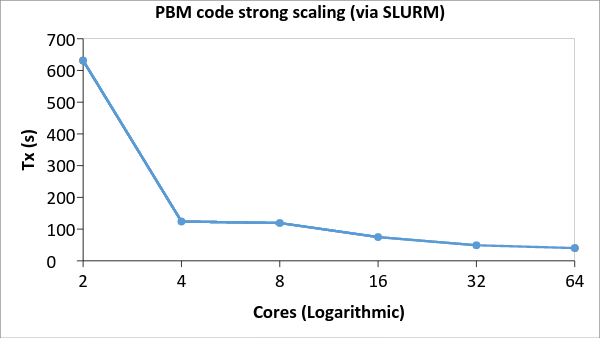
\includegraphics[scale=0.5]{rslts_strong_scale_slurm}
	      \caption{ PBM strong scale slurm}
	      %\caption{hello tesh}
	      \label{fig:rslts_pbm_strong_scale}
	      \end{figure}
	    \par 2. fig scaling w/ RP  
	      \begin{figure}[H]
	      \centering
	      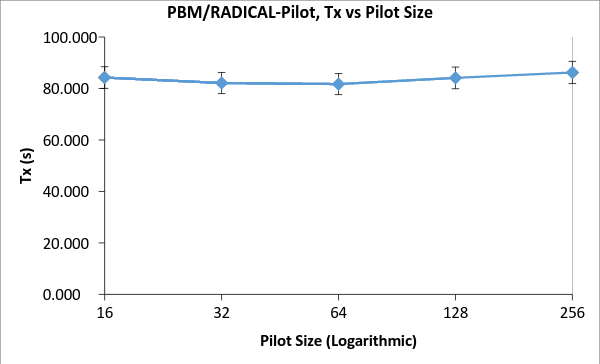
\includegraphics[scale=0.5]{rslts_pbmbyrp_strng}
	      \caption{ PBM strong scale RP}
	      %\caption{hello tesh}
	      \label{fig:rslts_pbmbyrp_strng}
	      \end{figure} 
	      
	    \subsubsection{Parallel PBM Parameter space and Parameter Estimation}
	     \par I. show how effective parallel pbm is for parameter estimation 
	     \par II. Find/ explore ranges of DEM data that PBM can use to find Critical parameters and sensitivities will be useful to us in linking and in picking best DEM parameters to vary and best parameters for PBM+DEM code 
	     \par 1. fig range of some parameters?
	     \par 2. fig range of other pbm parameter ?
	     
	%\begin{table}[h]
	%\caption{Parameters used in the Population Balance Model} %\label{table:rslts_pll_pbm}
	%\begin{center}
	%\begin{tabular}{c|c|c|c|c|c|c|c|c}
	%\hline
	%\bf{Cores in Parallel} &\bf{Num. MPI Proc.} &\bf{Threads/ MPI Proc.} &\bf{Wall %Time} &\bf{Speed Up} &\bf{Parallel Effic} &\bf{Pll. Wall Time/ Ser. Wall Time} %&\bf{Gran. Time/ Wall Time} &\bf{Speed Up w.r.t. Matlab}\\
	%\hline
	%$1$   & $1$  & $1$ & $222$ &  $1.00$  & $1.0 $  & $100$  & $246.67$ & $11.57$\\
	%$128$ & $16$ & $8$ & $6$   & $37.000$ & $0.289$ & $2.70$ & $\% 6.67$  & %$428.17$\\
	%\hline
	%\end{tabular}
	%\end{center}
	%\end{table}   
	   
	  
	  \subsection{DEM}
	    \subsubsection{DEM Spacial Decomposition Studies}
	    \par LIGGGHTS\textsuperscript{\textregistered} divides the work space into various sections and each section being sent to a core for calculation. Thus, the division of the space becomes an important criteria for the simulation for efficient load balancing. The initial stuides were undertaken for a mono-sized particle of size 1mm and the simulation was carried out for 0.5 seconds of wall time. The initial timing stuides for the decomposition were performed using 64 cores. The effect of the decomposition on the simulation time can be seen in Table \ref{table:rslts_dem_slicing_studies}. This indicates that dividing the x-direction in more number of compartments help increase the speed of the simulation. This is easy to comprehend since the granulator has its length parallel to the x-axis. These results also show that if the geometry is divided into more than 2 compartments in the y-axis or the z-axis the simulation time increases. This can be accounted to the increased communication required to transfer the rotating impeller mesh from one compartment in the y-axis or the z-axis to the another compartment for each time step. Since MPI is limited by communication in between the nodes, a speed decrease is observed due to increased partitioning in these directions.
	    
	      \begin{table}[ht]
	      %\centering
	      %\resizebox{\textwidth}{!}
	      \caption{The effect of spatial decomposition on the performance of the DEM simulations}
		  \label{table:rslts_dem_slicing_studies}
		  \begin{center}
		  \resizebox{\textwidth}{!}{\begin{tabular}{c|c|c|c}
		  \hline
		  \bf{Slices in x-direction}&\bf{Slices in y-direction}&\bf{Slices in z-direction}& Time taken for a 0.5 second simulation (in minutes)\\
		  \hline
		  
		  \end{tabular}}

\end{center}		  	      
	      \end{table}
	      
		  \par When MPI is used for parallelization of a task, load balancing becomes an important parameter that needs to be considered. Each processor used during the task is utilised with the similar usage as compared to other processors being used. Following the results from the initial timing studies,the y and the z-axes were not divided in more than 2 compartments for 128 and 256 core simulation as well. This meant that the x-axis was divided into 32 and 64 compartments respectively. In order to avoid the expensive communication between the processes, LIGGGHTS\textsuperscript{\textregistered} tries to insert the particles towards the centre of the compartment such that the number of ghost atoms are minimized. But, slicing in the x-axis reduced the space available for the insertion of the particles thus, many of the particles were inserted incorrectly. Another abnormal behaviour observed during these simulation was the particles halted at certain compartment and no particle travelled beyond this compartment in the x-direction. Thus, another set of timing studies were performed for the 128 and 256 core simulations. The comparison of simulation times have been shown in figure.
		  
		  \begin{figure}[H]
		  \centering		  	      
	      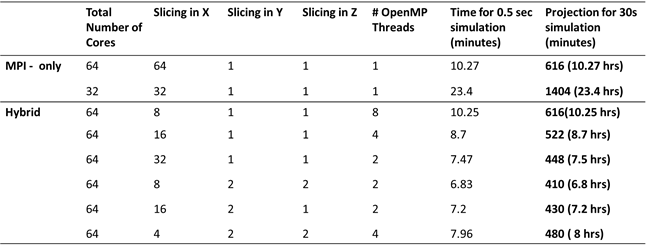
\includegraphics[scale=0.75]{slicing_studies.png}
	      \caption{ Slicing Studies}
	      \end{figure}
	    
	    \par fig vary PSD ( range and/or particle sizes) to see how $C_{coll}$ etc will be affected - important for PBM Kernel
	        
	    \par Talk about over-slicing or excess decomposition(confirm with profs)
	      \begin{figure}[H]
	      \centering
	      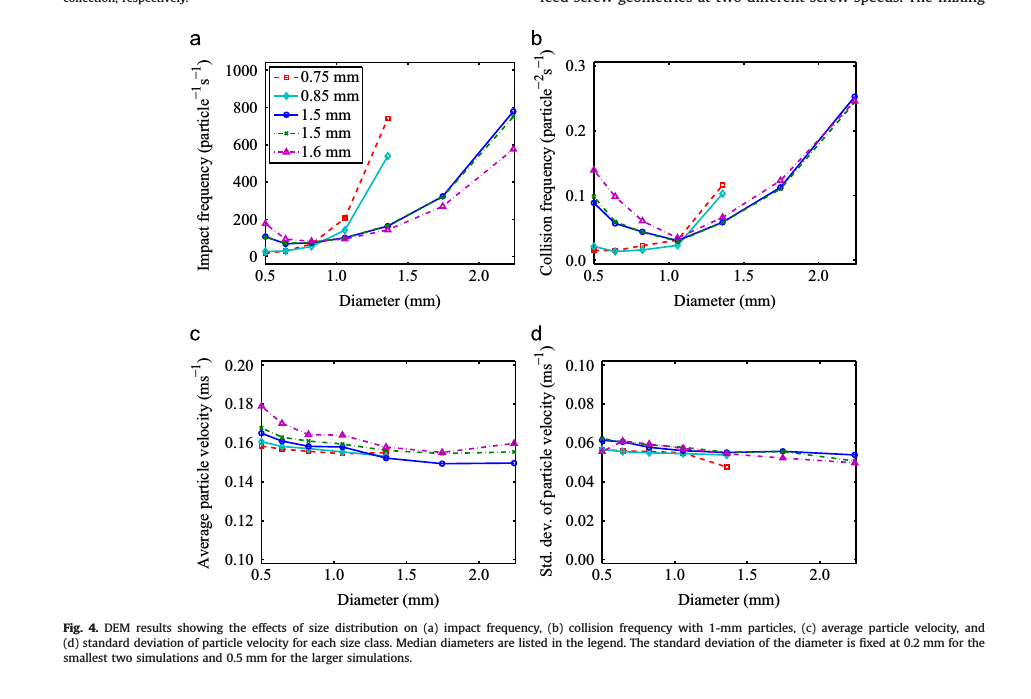
\includegraphics[scale=0.5]{rslts_dem_psd_velocity}
	      \caption{ fig from dana 2015 mechanistic bi-directional}
	      %\caption{hello tesh}
	      \label{fig:rslts_psd_velocity}
	      \end{figure}
	      
	      
	    \subsubsection{DEM Performance}
	    \par Talk about how the time for simulation varies with \# of cores
	    \par 1. fig scaling 
	      \begin{figure}[H]
	      \centering
	      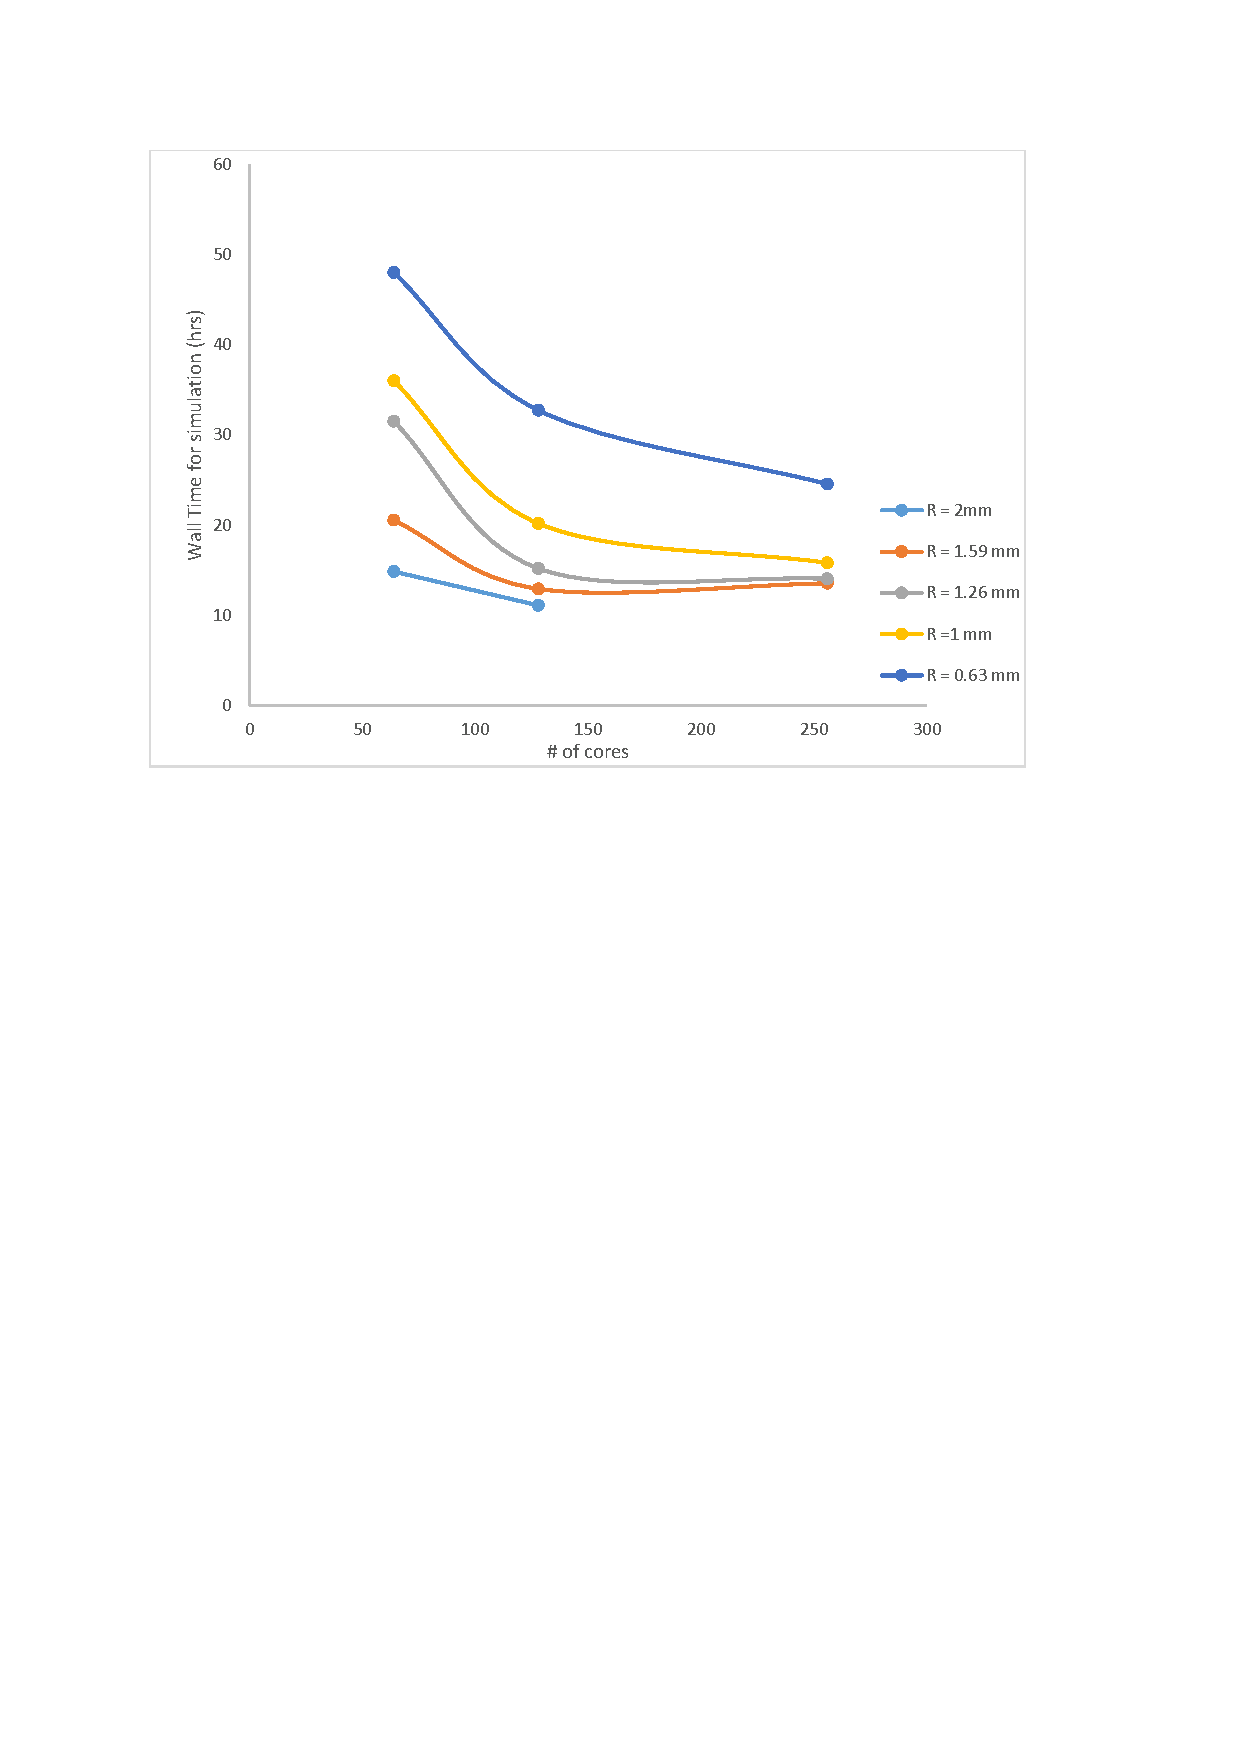
\includegraphics[scale=0.7]{timing_plot.pdf}
	      \caption{The variation in the amount of time taken for the simulation as a function of \# of cores}
	      %\caption{hello tesh}
	      \label{fig:rslts_DEM_strong_scale}
	      \end{figure}
	    \par 2. fig scaling w/ RP  
	      \begin{figure}[H]
	      \centering
	      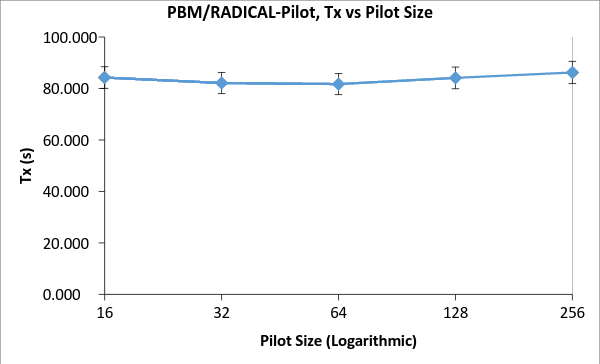
\includegraphics[scale=0.5]{rslts_pbmbyrp_strng}
	      \caption{ DEM scale with RP}
	      %\caption{hello tesh}
	      \label{fig:rslts_dembyRP_strng}
	      \end{figure}
	      
	    %\subsubsection{DEM Parameter Space} 
	 
	    
	  \subsection{PBM+DEM - RP} 
	    \subsubsection{PBM+DEM Validation/Accuracy?}
	   	\par Talk about how the physics remain the same whether mono-sized particles are used or a size distribution is used.
	   \par Figs comparing the one-way coupling from both these sources.
	    
	    \subsubsection{PBM+DEM Performance}
	    \par strong scaling
	    \par fig PBM + DEM RP strong scaling 
	      \begin{figure}[!htb]
	      \centering
	      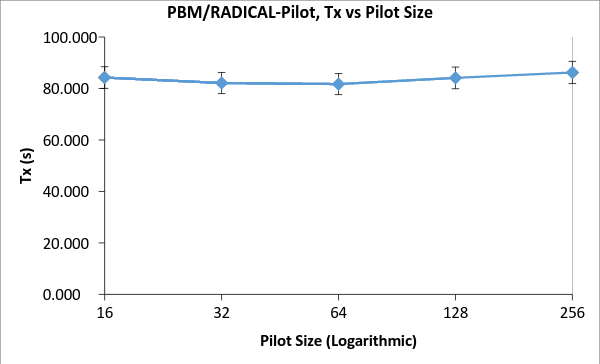
\includegraphics[scale=0.5]{rslts_pbmbyrp_strng}
	      \caption{PBM+DEM scale with RP}
	      %\caption{hello tesh}
	      \label{fig:rslts_dembyRP_strng}
	      \end{figure}
	
	    %\par weak scaling
	    %\par fig PBM + DEM RP weak scaling
	
	
	   \subsubsection{PBM+DEM Parameter studies}
	   \par show how PBM+DEM captures multi-physics as parameters changed. helps validate and support model development. show we have made a useful tool for future work.
	   \par fig 
	      \begin{figure}[H]
	      \centering
	      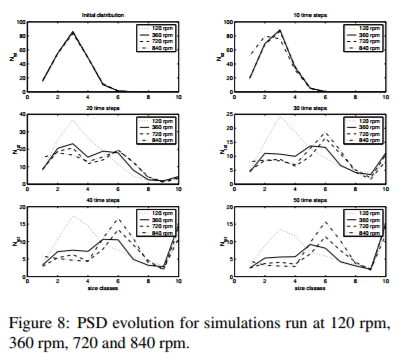
\includegraphics[scale=0.7]{rslts_psd_evo_time}
	      \caption{PBM+DEM scale with RP}
	      %\caption{hello tesh}
	      \label{fig:rslts_psd_evo_time}
	      \end{figure}
	    
	\section{Conclusions}
	
	\section*{References} 
	\bibliographystyle{elsarticle-harv}
	\bibliography{Bibli,radical_publications}
	\end{document}
